\documentclass[10pt, oneside]{article} 
\usepackage{amsmath, amsthm, amssymb, calrsfs, wasysym, verbatim, bbm, color, graphics, geometry}
\usepackage{graphicx}
\usepackage{float}
\usepackage{longtable}
\usepackage{rotating}
\usepackage{adjustbox}
\usepackage{booktabs}
\usepackage{caption}
\usepackage[english]{babel}
\usepackage[utf8]{inputenc}
\usepackage[table]{xcolor}
\usepackage{multicol}
\usepackage{hyperref}

\geometry{tmargin=.75in, bmargin=.75in, lmargin=.75in, rmargin = .75in}  

\newcommand{\R}{\mathbb{R}}
\newcommand{\C}{\mathbb{C}}
\newcommand{\Z}{\mathbb{Z}}
\newcommand{\N}{\mathbb{N}}
\newcommand{\Q}{\mathbb{Q}}
\newcommand{\Cdot}{\boldsymbol{\cdot}}

\newtheorem{thm}{Theorem}
\newtheorem{defn}{Definition}
\newtheorem{conv}{Convention}
\newtheorem{rem}{Remark}
\newtheorem{lem}{Lemma}
\newtheorem{cor}{Corollary}


\title{Computing Infrastructure: [Course Code]}
\author{[Sofia Martellozzo]}
\date{Academic Year 2021-2022}

\begin{document}

\maketitle
\newpage
\tableofcontents

\vspace{.25in}
\newpage

\section{Computing Infrastructure}

\subsection{Introduction}
\begin{defn}
{\bf Computing Infrastructure}: Technological infrastructure that provides hardware and software for computation to other systems and services.
\end{defn}


\begin{figure}[H]
    \begin{center}
    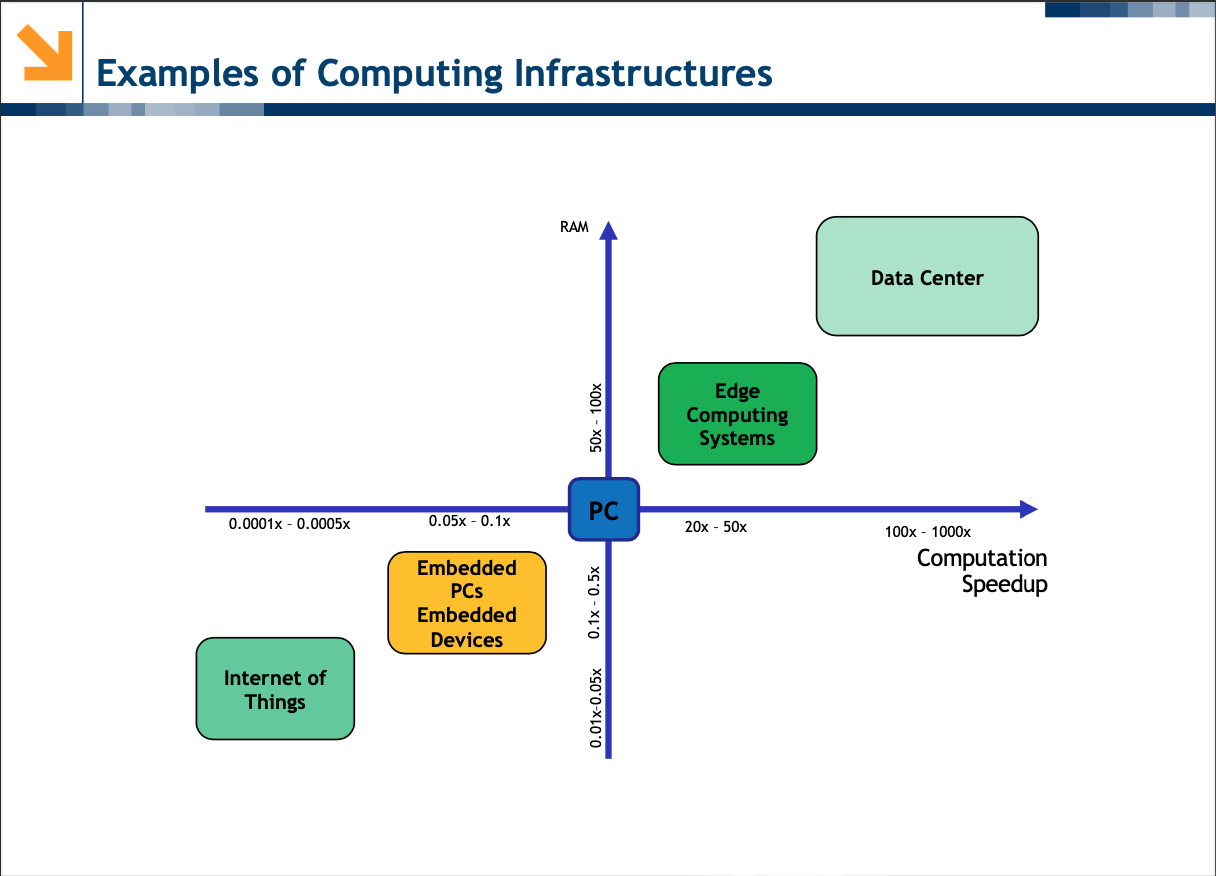
\includegraphics[width=0.5\textwidth]{img/img1.png}
    \caption{Computing Infrastructure}
    \label{fig:computing infrastructure}
    \end{center}
\end{figure}

\begin{multicols}{2}
\noindent
{\bf Advantages}:
\begin{itemize}
    \item Lower IT costs
    \item High performance
    \item Instant software updates
    \item “Unlimited” storage capacity
    \item Increased data reliability
    \item Universal document access
    \item Device Independence 
\end{itemize}

\columnbreak
\noindent
{\bf Disadvantages}:
\begin{itemize}
    \item Require a constant Internet connection
    \item Do not work well with low-speed connections
    \item Hardware Features might be limited
    \item Privacy and security issues
    \item High Power Consumption (1\% overall worldwide total energy consumption due to datacenters)
    \item Latency in making decision
\end{itemize}

\end{multicols}


\begin{figure}[H]
    \begin{center}
    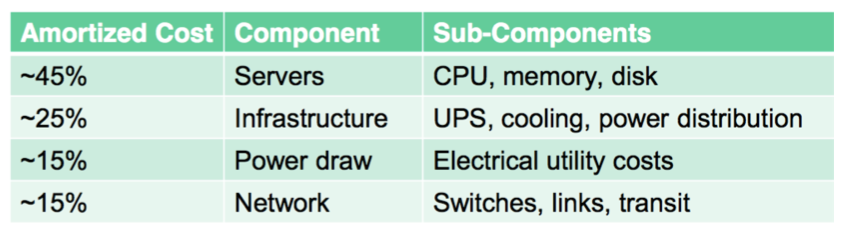
\includegraphics[width=0.5\textwidth]{img/img2.png}
    \label{fig:consumptions}
    \end{center}
\end{figure}

\newpage

%------------------------------------------------------%
\section{Data WareHouse}

\subsection{Introduction}
In the last few decades, computing and storage have moved from PC- like clients to smaller, often mobile, devices, combined with large internet services.\\
Traditional enterprises are also shifting to Cloud computing.
\begin{figure}[H]
    \begin{center}
    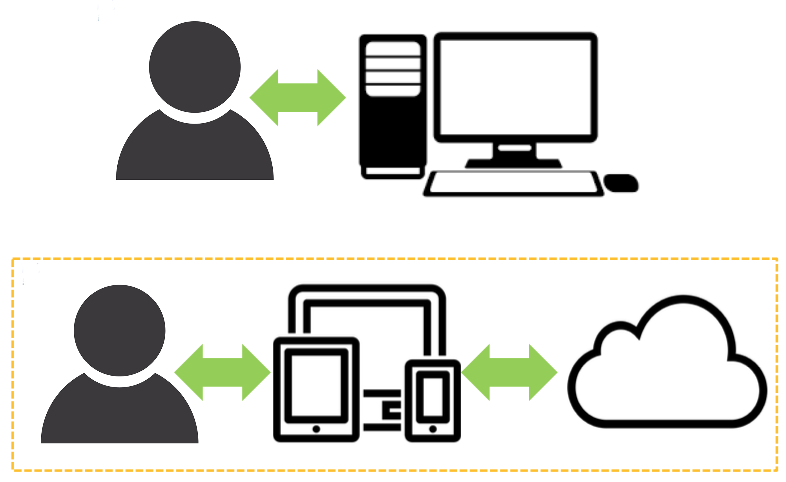
\includegraphics[width=0.5\textwidth]{img/img3.png}
    \label{fig:computing and storage}
    \end{center}
\end{figure}

\begin{multicols}{3}
\noindent
{\bf User experience improvements}
\begin{itemize}
    \item Ease of management (no configuration or backups needed)
    \item Ubiquity of access
\end{itemize}

\columnbreak
\noindent
{\bf Advantages to vendors}
\begin{itemize}
    \item Software-as-a-service allows faster application development (easier to make changes and improvements)
    \item Improvements and fixes in the software are easier inside their data centers (instead of updating many millions of clients with peculiar hardware and software configurations)
    \item The hardware deployment is restricted to a few well-tested configurations.
\end{itemize}

\columnbreak
\noindent
{\bf Server-side computing allows}
\begin{itemize}
    \item Faster introduction of new hardware devices (e.g., HW accelerators or new hardware platforms)
    \item Many application services can run at a low cost per user.
\end{itemize}

\end{multicols}
Some workloads require so much computing capability that they are a more natural fit in datacenter (and not in client-side computing).\\
A couple of examples (Search services (web, images, and so on), Machine and Deep Learning (\href{https://www.theguardian.com/commentisfree/2020/sep/08/robot-wrote-this-article-gpt-3}{GPT-3}).

\subsection{From Data Centers to Warehouse-scale computers}
{\bf Data centers} = is a place in which there are many servers\\
{\bf Whareouse} = is a type of Data Center, it works as a computer.\\
The trends toward server-side computing and widespread internet services created a new class of computing systems:
\begin{defn}
{\bf warehouse-scale computers (WSCs)}The massive scale of the software infrastructure, data repositories, and hardware platform.
\begin{itemize}
    \item is an internet service (= service provided by inyternet)
    \item may consist of tens or more individual programs (= not a single program, a collection of them that together create/provide the service)
    \item such programs interact to implement complex end-user services such as email, search, maps or machine learning.
\end{itemize}
\end{defn}
Data centers are buildings where multiple servers and communication units are co-located because of their common environmental requirements and physical security needs, and for ease of maintenance.\\
In {\bf Traditional Data Center}: typically host a large number of relatively small- or medium-sized applications, each applications is running on a dedicated hardware infrastructure that is de-coupled and protected from other systems in the same facility, applications tend not to communicate each other. Those data centers host hardware and software for multiple organizational units or even different companies.
\begin{figure}[H]
    \begin{center}
    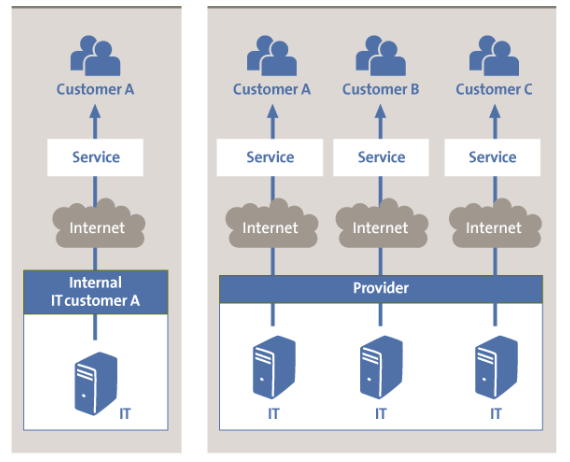
\includegraphics[width=0.3\textwidth]{img/img4.png}
    \caption{Traditional Data Center}
    \label{fig:Traditional Data Center}
    \end{center}
\end{figure}
{\bf WSCs} belong to a single organization, use a relatively homogeneous hardware and system software platform (=> easier to manage and cheaper, but has limitations on functionalities), and share a common systems management layer (such as Google, Facebook, Alibaba, Amazon, Dropbox...).\\
(you have 1 services that you want to provide to a 'huge' amount of customers)\\
Run a smaller number of very large applications (or internet services).\\
The common resource management infrastructure allows significant deployment flexibility.\\
The requirements of:
\begin{itemize}
    \item homogeneity
    \item single-organization control
    \item cost efficiency
\end{itemize}
\begin{figure}[H]
    \begin{center}
    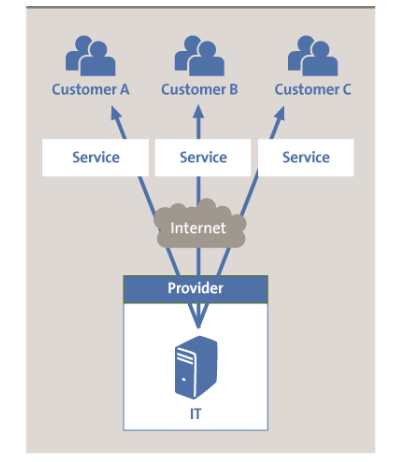
\includegraphics[width=0.25\textwidth]{img/img5.png}
    \caption{Warehouse-Scale Computers}
    \label{fig:WSCs}
    \end{center}
\end{figure}
Initially designed for online data-intensive web workloads, WSCs also now power public clouds computing systems (e.g., Amazon, Google, Microsoft). Such public clouds do run many small applications, like a traditional data center. (All of these applications rely on Virtual Machines (or Containers), and they access large, common services for block or database storage, load balancing, and so on, fitting very well with the WSC model).\\
These are not just a collection of servers: \\The software running on these systems executes on clusters of hundreds to thousands of individual servers (far beyond a single machine or a single rack)\\
+ \\The machine is itself this large cluster or aggregation of servers and needs to be considered as a single computing unit. (=$>$ scale up in terms of performance)\\
{\bf Several data-centers}:
Multiple Data Center located far apart (placed near point of interest) => becomes important also the PRIVACY: data of a country must remain in it.\\
Multiple data centers are (often) replicas of the same service (to reduce user {\bf latency} and improve serving {\bf throughput}).\\
A request is typically fully processed within one data center.\\
{\bf Availability}:
Services provided through WSCs must guarantee high availability, typically aiming for at least 99.99\% uptime (i.e., one-hour downtime per year). Achieving such fault-free operation is difficult when a large collection of hardware and system software is involved.\\
WSC workloads must be designed to gracefully tolerate large numbers of component faults with little or no impact on service level performance and availability.

\subsection{Architectural Overview of WSCs}
Hardware implementation of WSCs might differ significantly each other; However, the architectural organization of these systems is relatively stable.
\begin{multicols}{2}
\begin{figure}[H]
    \begin{center}
    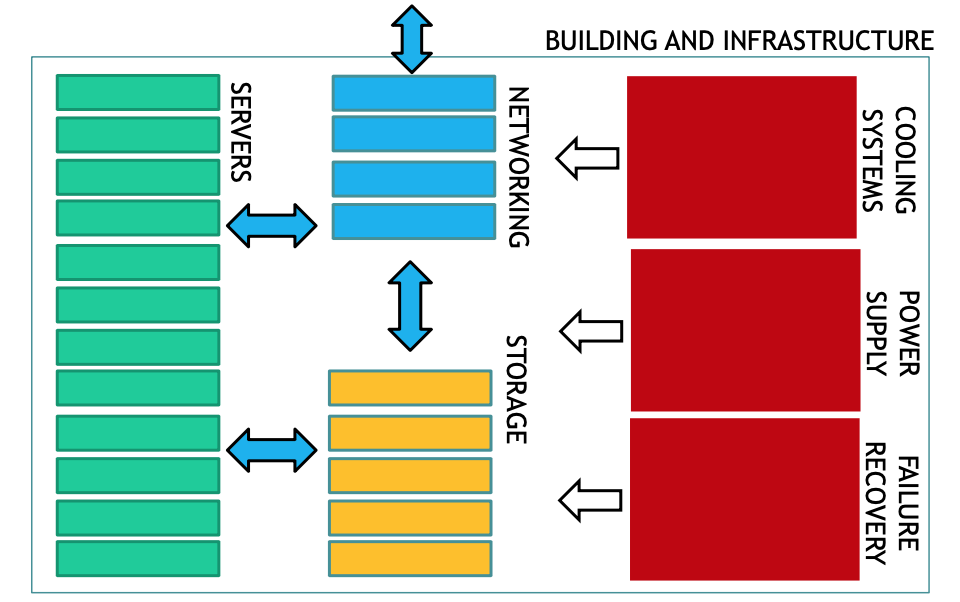
\includegraphics[width=0.4\textwidth]{img/img6.png}
    \caption{Warehouse-Scale Computers Overview}
    \label{fig:WSCs overview}
    \end{center}
\end{figure}
\columnbreak
\begin{figure}[H]
    \begin{center}
    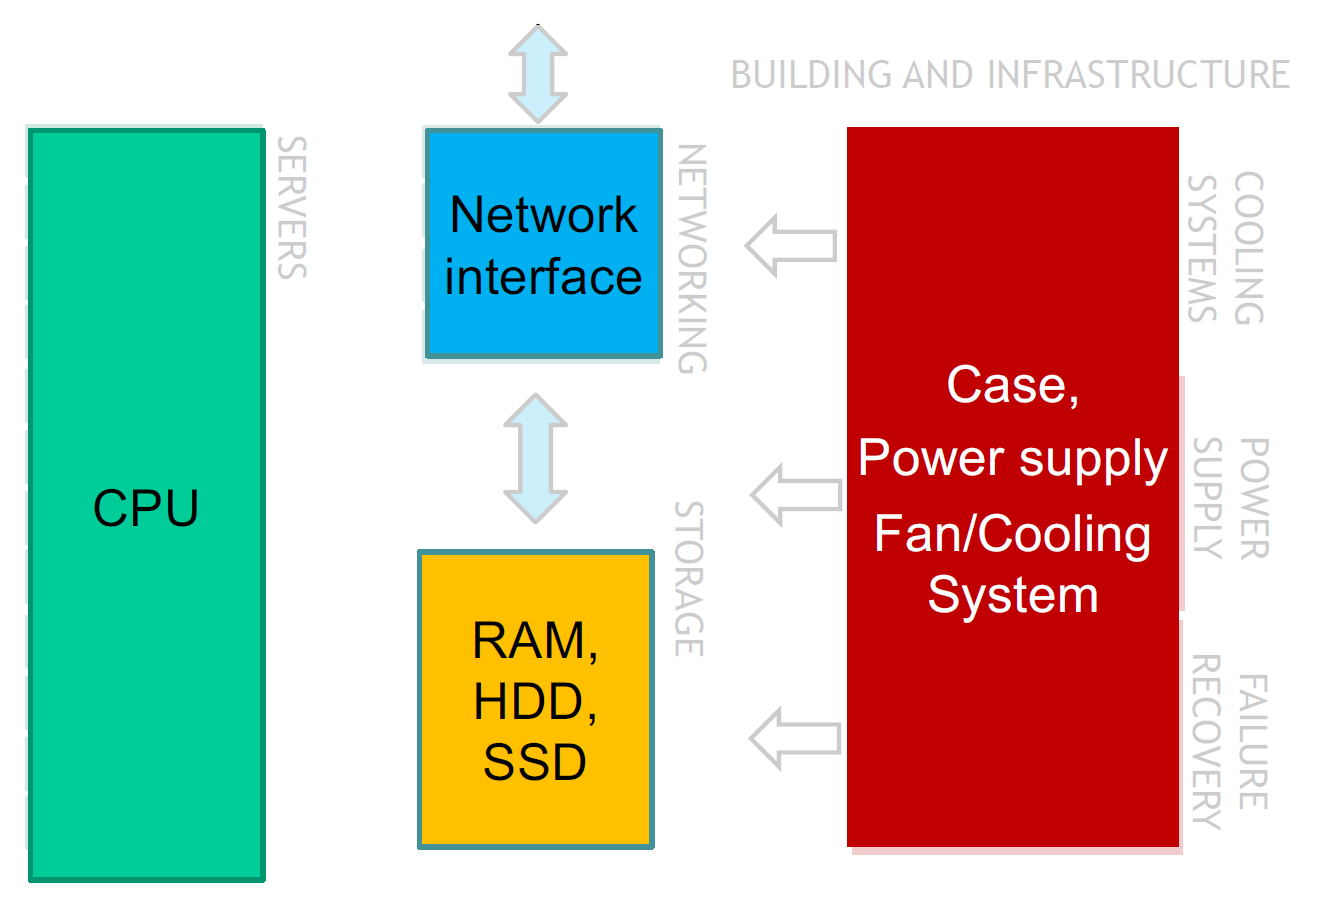
\includegraphics[width=0.4\textwidth]{img/img7.png}
    \caption{}
    \label{fig:WSCs overview2}
    \end{center}
\end{figure}
\end{multicols}

\begin{itemize}
    \item \color{green}\textbf{Servers}\color{black}
    : the main processing equipment
    
    \item \color{yellow}\textbf{Storage}\color{black}
    : how and where to store the information
    \item \color{blue}\textbf{Networking}\color{black}
    : providing internal and external connections
    \item \color{red}\textbf{Building and Infrastructure}\color{black}
    :WSC has other important components related to power delivery, cooling, and building infrastructure that also need to be considered
\end{itemize}




%------------------------------------------------------%
\newpage
\section{Server}
\subsection{Overview}
Servers hosted in individual shelves are the basic building blocks of WSCs. They are interconnected by hierarchies of networks, and supported by the shared power and cooling infrastructure. They are stored in  shelves called wraks, that are organized along corridors. All servers are connected to each other in the same wrak, but also (on a higher level) communicate through different wrack.
 They have 3 type of shape:
    \begin{itemize}
        \item Rack (1U or more)
        \item Blade enclosure format 
        \item Tower
    \end{itemize} 
    They may differ in: 
    \begin{itemize}
        \item Number and type of CPUs.
        \item Available RAM Locally attached disks (HDD, SSD or not installed).
        \item Other special purpose devices (like GPUs, DSPs and coprocessors).
    \end{itemize}  
and are usually built in a tray or blade enclosure format, housing the motherboard, chipset, additional plug-in components.

\subsubsection{The Motherboard}
The motherboard provides sockets and plug-in slots to install CPUs, memory modules (DIMMs), local storage (such as Flash SSDs or HDDs), and network interface cards (NICs) to satisfy the range of resource requirements.
\subsubsection{Chipset and additional components}
\begin{itemize}
    \item Number and type of CPUs:
\begin{itemize}
    \item From 1 to 8 CPU socket
    \item Intel Xeon Family, AMD EPYC, etc..
\end{itemize}
    \item Available RAM
    \begin{itemize}
        \item From 2 to 192 DIMM Slots
    \end{itemize}
    \item Locally attached disks:
    \begin{itemize}
        \item From 1 to 24 Drive Bays
        \item HDD or SSD (see specific lecture)
        \item SAS (higher performance but more expensive) or SATA (for entry level servers, usually cheaper)
    \end{itemize}
    \item Other special purpose devices:
    \begin{itemize}
        \item From 1 to 20 GPUs per node, or TPUs
        \item NVIDIA Pascal, Volta, etc..
    \end{itemize}
    \item Form factor:
    \begin{itemize}
        \item Form 1U to 10U
        \item Tower
    \end{itemize}
\end{itemize}
We distinguish between rack, tower and blade.

\subsubsection{Rack}
Racks are special shelves that accommodate all the IT equipment and allow their interconnection. The rack are used to store many {\bf Rack server}.\\ 
IT equipment must conform to specific sizes to fit into the rack shelves. Them has different hight, but same SIZE, that is {\bf standardize} (so make them easier to design): server racks are measured in rack units "U's".\\ The advantages of using these racks is that it allows designers to stack up (one on top of the others) other electronic devices along with the servers.\\
\newline
A Rack is not only a physical structure:
\begin{multicols}{2}
\noindent
\begin{figure}[H]
    \begin{center}
    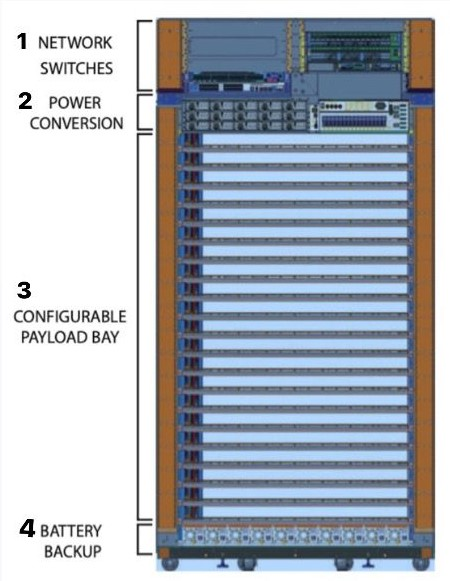
\includegraphics[width=0.4\textwidth]{img/img8.jpeg}
    \caption{RACK Servers}
    \label{fig:RACK servers}
    \end{center}
\end{figure}
\columnbreak
\noindent
(3) The rack is the shelf that holds tens of servers together. \\(2-4) It handles shared power infrastructure, including power delivery, battery backup, and power conversion.\\
(2) There are 2 types of electronic delivery: it can provide/automatically select the server (can swich ON and OFF remotely the servers).\\
(4) It is used in case of problems with energy (power failure):
\begin{itemize}
    \item just swich off if a power failure occur, them cannot supply all the power demand (execution)
    \item it provides 15 minutes of power, that is the time to swich on the power supply generator (source) 
\end{itemize}
(3) The width and depth of racks vary across WSCs: some are classic 19-in wide, 48-in deep racks, while others can be wider or shallower.\\ 
(1) It is often convenient to connect the network cables at the top of the rack, such a rack-level switch is appropriately called a Top of Rack (TOR) switch.
\end{multicols}

Rack servers:\\
It is designed to be positioned in a bay, by vertically stacking servers one over the another along with other devices
\begin{multicols}{2}
\noindent
{\bf \color{green}Pros}\color{black}
\begin{itemize}
    \item {\bf Failure containment}: very little effort to identify, remove, and replace a malfunctioning server with another.
    \item {\bf Simplified cable management}: easy
and efficient to organize cables.
    \item {\bf Cost-effective}: Computing power and efficiency at relatively lower costs.
\end{itemize}
\columnbreak
\noindent
{\bf \color{red}Cons}\color{black}
\begin{itemize}
    \item {\bf Power usage}: Needs of additional cooling systems due to their high overall component density, thus consuming more power.
    \item {\bf Maintenance}: Since multiple devices are placed in racks together, maintaining them gets considerably tough with the increasing number of racks.
\end{itemize}
\end{multicols}
\newpage
\subsubsection{Tower}
It is the simplest but is not usually adopted.
\textbf{Tower Servers}
look and feel a lot like traditional tower PCs.
Like everything they have their Pros and Cons.
\begin{multicols}{2}
\noindent
{\bf \color{green}Pros}\color{black}
\begin{itemize}
    \item {\bf Scalability and ease of upgrade}: customized and upgraded based on necessity.
    \item {\bf Cost-effective}: Tower servers are probably the cheapest of all kinds of servers
    \item {\bf Cools easily}: Since a tower server has a low overall component density, it cools down easily.
\end{itemize}
\columnbreak
\noindent
{\bf \color{red}Cons}\color{black}
\begin{itemize}
    \item {\bf Consumes a lot of space}: These servers are difficult to manage physically.
    \item {\bf Provides a basic level of performance}: a tower server is ideal for small businesses that have a limited number of clients.
    \item {\bf Complicated cable management}: devices aren't easily routed together
\end{itemize}
\end{multicols}

  
\subsubsection{Blade}
Blade servers are the latest and the most advanced type of servers in the market. They can be termed as hybrid rack servers (like orizontal rack server but placed vertically), in which servers are placed inside blade enclosures, forming a blade system. The biggest advantage of blade servers is that these servers are the smallest types of servers available at this time and are great for conserving space. A blade system also meets the IEEE standard for rack units and each rack is measured in the units of “U’s”.
\begin{multicols}{2}
\noindent
{\bf \color{green}Pros\color{black}}
\begin{itemize}
    \item {\bf Load balancing and failover}: Thanks to its much simpler and slimmer infrastructure, load balancing among the servers and failover management tends to be much simpler.
    \item {\bf Centralized management}: In a blade server, you can connect all the blades through a single interface, making the maintenance and monitoring easy.
    \item {\bf Cabling}: Blade servers don't involve the cumbersome tasks of setting up cabling. Although you still might have to deal with the cabling, it is near to negligible when compared to tower and rack servers.
    \item {\bf Size and form-factor}: They are the smallest and the most compact servers, requiring minimal physical space.
\end{itemize}
\columnbreak
\noindent
{\bf \color{red}Cons}\color{black}
\begin{itemize}
    \item {\bf Expensive configuration}: Although upgrading the blade server is easy to handle and manage, the initial configuration or the setup might require heavy efforts in complex environments.
    \item {\bf HVAC}: Blade servers are very powerful and come with high component density. Therefore, special accommodations have to be arranged for these servers in order to ensure they don't get overheated. Heating, ventilation, and air conditioning systems must be managed well in the case of blade servers.
\end{itemize}
\end{multicols}

\subsection{Data-center architecture}
The IT equipment is stored into corridors and organized into racks (the goal is to maximize the number of racks => max number of servers).\\
Corridors where servers are located are split into \emph{cold aisle}, where the front panels of the equipment is reachable, and \emph{warm aisle} where the back connections are located.\\
{\bf cooling system}: Cold air flows from the front (cool aside), cools down the equipment, and leave the room from the back (warm aide). There is an additional roof in order to do not waste cold air on the Back side (cold part of the corridor).
\newline
\subsection{Hardware accelerators}
Hardware accelerator are accurate particular applications that support specific high operation (of ML) with a lot of data.
Deep learning models began to appear and be widely adopted, enabling specialized hardware to power a broad spectrum of machine learning solutions. To satisfy the growing compute needs for deep learning, WSCs deploy specialized accelerator hardwares:
\begin{itemize}
    \item GPU
    \item TPU
    \item FPGA
\end{itemize}
\subsubsection{Graphical Processing Units (GPU)}
\textbf{Data-parallel computations:}
the same program is executed on many data elements in parallel. The scientific codes are mapped onto the matrix operations. High level languages (such as CUDA, OpenCL, OPENACC, OPENMP, SYCL) are required. Up to 1000x faster than CPU.
\begin{figure}[H]
    \begin{center}
    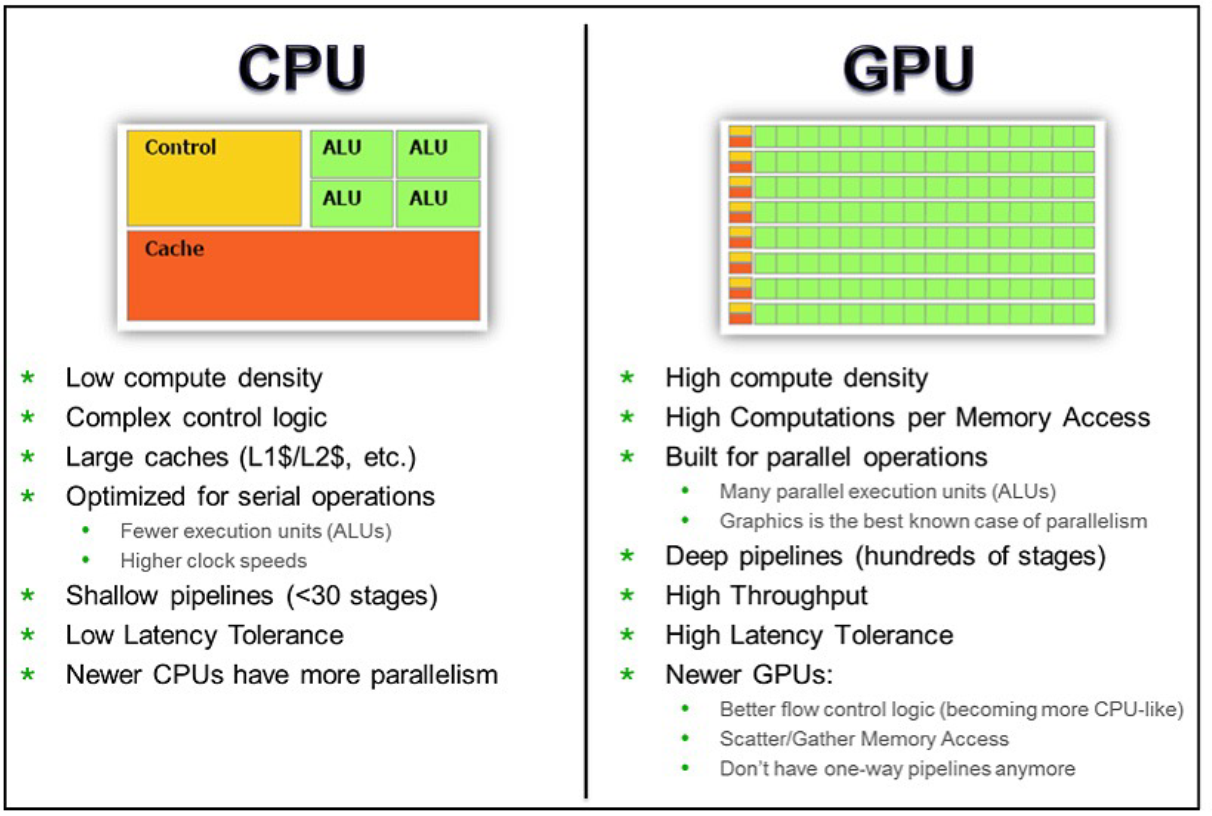
\includegraphics[width=0.4\textwidth]{img/img9.png}
    \caption{CPU vs GPU}
    \label{fig:CPU vs GPU}
    \end{center}
\end{figure}
The performance of such a synchronous system is limited by the slowest learner and slowest messages through the network. Since the communication phase is in the critical path, a high performance network can enable fast reconciliation of parameters across learners.\\
\textbf{GPUs within the rack: PCI AND NVlink}
GPUs are configured with a CPU host connected to a PCIe-attached accelerator tray with multiple GPUs.\\GPUs within the tray are connected using high-bandwidth interconnects such as NVlink.\\
\textbf{NVLINK evolution and NVSwitch}
In the A100 GPU, each NVLink lane supports a data rate of 50x 4 Gbit/s in each direction. The total number of NVLink lanes increases from six lanes in the V100 GPU to 12 lanes in the A100 GPU, now yielding 600 GB/s total
\subsubsection{Tensor Processing Unit (TPU)}
While suited to ML, GPUs are still relatively general purpose devices. In recent years, designers further specialized them to ML-specific hardware: Custom-built integrated circuit developed specifically for machine learning and tailored for TensorFlow.\\
\begin{multicols}{2}
    A Tensor is an n-dimensional matrix. This is the basic unit of operation in with TensorFlow.\\TPUs are used for training and inference:
\begin{itemize}
    \item TPUv1 is an inference-focused accelerator connected to the host CPU through PCIe links.
    \item Differently, TPUv2 and TPV3 focus training and inference
\end{itemize}
    Each Tensor core has an array for matrix computations (MXU) and a connection to high bandwidth memory (HBM) to store parameters and intermediate values during computation.
    \textbf{TPUv2}
    \\
    8 GiB of HBM for each TPU core, one MXU for each TPU core, 4 chips, 2 cores per chip.
    \columnbreak
    \noindent
    \begin{figure}[H]
        \begin{center}
        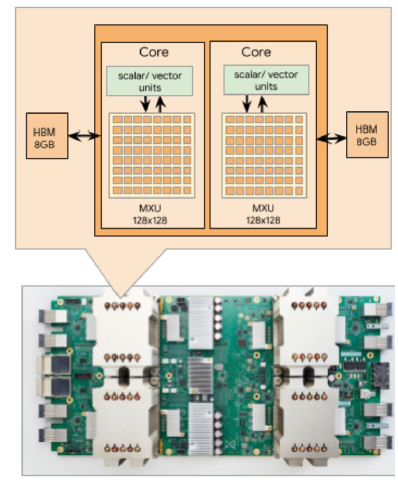
\includegraphics[width=0.28\textwidth]{img/img10.png}
        \caption{TPUv2 - 4 chips, 2 core per chip}
        \label{fig:TPUv2 - 4 chips, 2 core per chip}
        \end{center}
    \end{figure} 
\end{multicols}

In a rack multiple TPUv2 accelerator boards are connected through a custom high-bandwidth network to provide 11.5 petaflops of ML compute.\\
The high bandwidth network enables fast parameter reconciliation with well-controlled tail latencies.\\ Up to 512 total TPU cores and 4 TB of total memory in a TPU Pod (64 units).\\
\textbf{TPUv3} is the first \textbf{liquid-cooled accelerator}
in Google’s data center (here there is no fresh air to cool it down, used fresh liquid). 2.5x faster than TPUv2. Such supercomputing-class computational power supports new ML capabilities (e.g., AutoML), and rapid neural architecture search. The v3 TPU Pod provides a maximum configuration of 256 devices for a total 2048 TPU v3 cores, 100 petaflops and 32 TB of TPU memory.\\
\textbf{TPUv4} announced June 2021, used to support Google services (not yet available as a cloud service).One v4 TPU pod includes 4096 devices: About 2.7x faster than TPUv3 and same computing capacity as 10
millions of laptops. 


\subsubsection{Field-Programmable Gate Array (FPGA)}
Array of logic gates that can be programmed (“configured”) in the field, i.e.,by the user of the device as opposed to the people who designed it.\\ Array of carefully designed, and interconnected digital subcircuits, that efficiently implement common functions offering very high levels of flexibility. The digital subcircuits are called configurable logic blocks (CLBs).\\VHDL and Verilog are hardware description languages (HDLs), that allow to “describe” hardware. HDL code is more like a schematic that uses text to introduce components and create interconnections.\\Microsoft deployed FPGAs inside its Datacenters.
\begin{figure}[H]
    \begin{center}
    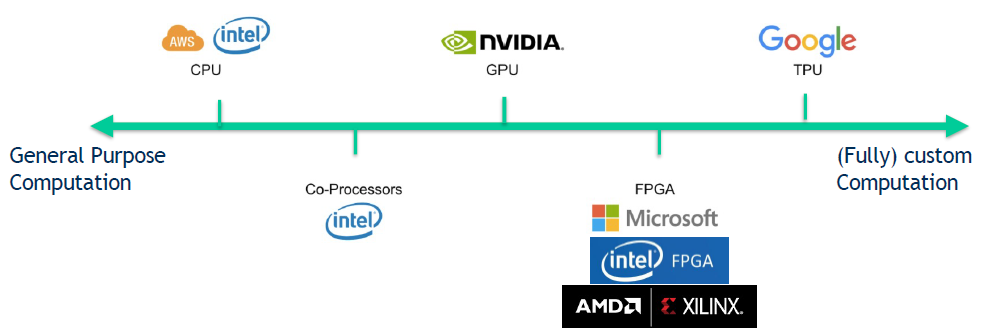
\includegraphics[width=0.4\textwidth]{img/img11.png}
    \caption{Overview}
    \label{fig:Overview}
    \end{center}
\end{figure}
\subsubsection{Advantages and Disadvantages}
\textbf{CPU}
\begin{itemize}
    \item {\bf Advantages}:Easy to be programmed and support any programming framework.\\ Fast design space exploration
    and run your applications.
    \item {\bf Disadvantages}: Most suited for simple AI models that do not take long to train and for small models with small training set.
\end{itemize}
\textbf{GPU}
\begin{itemize}
    \item {\bf Advantages}:Ideal for applications in which data need to be processed in parallel like the pixels of images or videos.
    \item {\bf Disadvantages}: Programmed in languages like CUDA and OpenCL and therefore provide limited flexibility compared to CPUs.
\end{itemize}
\textbf{TPU}
\begin{itemize}
    \item {\bf Advantages}:Very fast at performing dense vector and matrix computations and are specialized on running very fast program based on Tensorflow.
    \item {\bf Disadvantages}: For applications and models based on the TensorFlow. Lower flexibility compared to CPUs and GPUs.
\end{itemize}
\textbf{FPGA}
\begin{itemize}
    \item {\bf Advantages}:Higher performance, lower cost and lower power consumption compared to other options like CPUs and GPU.
    \item {\bf Disadvantages}: Programmed using OpenCL and High-level Synthesis (HLS).\\Limited flexibility compared to
    other platforms.
\end{itemize}
\newpage

%----------------------------------------%
\section{Storage}
Nowadays machines generate data at an unprecedented rate 


\begin{itemize}
        \item Disks and Flash SSDs are the building blocks of today’s WSC storage systems.
        \item These devices are connected to the data-center network and managed by sophisticated distributed systems
    \end{itemize} 
Examples: 
\begin{itemize}
    \item Direct Attached Storage (DAS)
    \item Network Attached Storage (NAS)
    \item Storage Area Networks (SAN)
    \item RAID controllers
\end{itemize}

\subsection{Hard Disk Drives}
\begin{multicols}{2}
A hard disk drive (HDD) is a data storage using rotating disks (platters) coated with magnetic material.\\
Data is read in a random-access manner, meaning individual blocks of data can be stored or retrieved in any order rather than sequentially.\\
An HDD consists of one or more rigid ("hard") rotating disks (platters) with magnetic heads arranged on a moving actuator arm to read and write data to the surfaces.\\
The {\bf Sector} is where you read and/or write; The organization of the data is in order to minimize the movement of the head (that increase the seek time): place the data that are related near! If the head continues to go forward and back increase the Latency!
\columnbreak
\begin{figure}[H]
    \begin{center}
    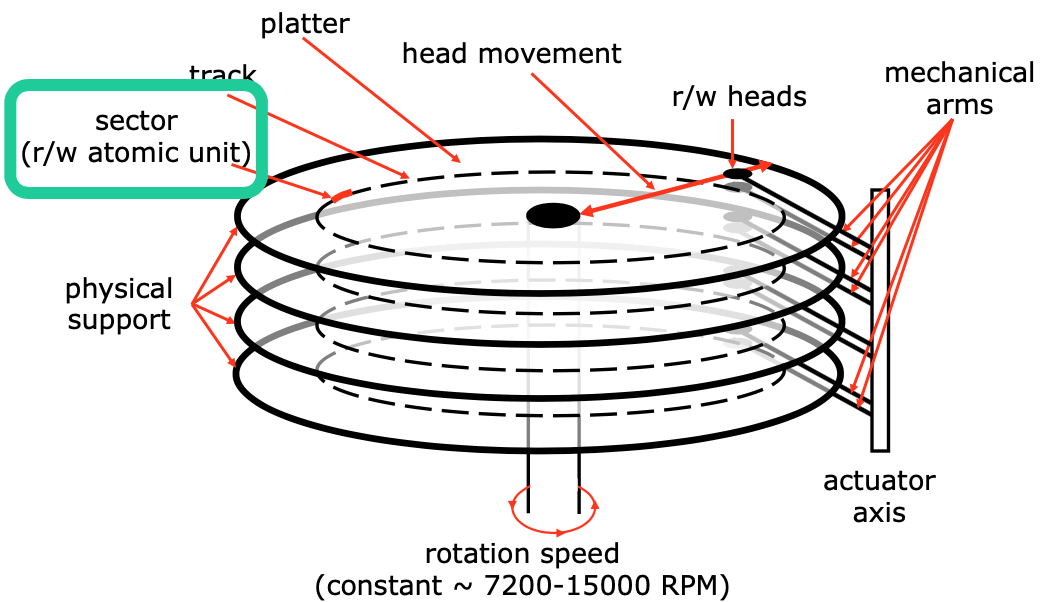
\includegraphics[width=0.5\textwidth]{img/img12.png}
    \caption{Hard Disk}
    \label{fig:HDD}
    \end{center}
\end{figure}
\end{multicols}
\subsubsection{Read Write heads, basic characteristic}
\begin{itemize}
    \item float on a film of air (tens of nanometers) above the platters
    \item one head for each magnetic platter
    \item cylinder: set of tracks with the same radius
    \item {\bf seek time}: time required to reach the track that contains the data, 3$\div$14 ms
\end{itemize}
\subsubsection{Other characteristics}
\begin{itemize}
    \item Diameter: about 9 cm (3,5$\div$2.5 in) - two surfaces
    \item Rotation speed: 7200$\div$15000 RPM round per minute
    \item Track density: 16,000 TPI (Track Per Inch)
    \item Sectors: 512 Byte (usually), but might be different (are numbered sequentially, have a header and an error correction code)
    \item Heads: can be parked close to the center or to the outer diameter (mobile drives)
    \item Disk buffer cache: embedded memory in a hard disk drive that has the function of a buffer between the disk and the computer (several MB)
\end{itemize}

\begin{figure}[H]
    \begin{center}
    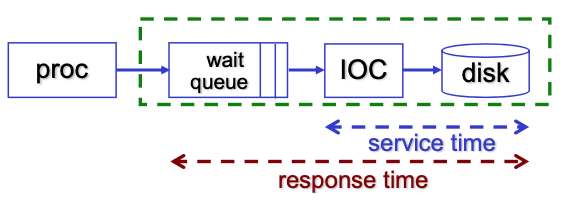
\includegraphics[width=0.5\textwidth]{img/img13.png}
    \caption{HDD service and response time}
    \label{fig:HDD time}
    \end{center}
\end{figure}
{\bf Service Time}\\
$s_{disk}$: seek time + rotational latency + data transfer time + controller overhead
\begin{itemize}
    \item {\bf seek} time: head movement time ($\approx$ ms), is a function of the number of cylinders traversed
    \item {\bf latency} time: time to wait for the sector ($\approx$ ms, $\frac{1}{2}$ round)
    \item {\bf transfer} time: is a function of rotation speed, storing density, cylinder position ($\approx$ MB/sec)
    \item {\bf controller overhead}: buffer management (data transfer) and interrupt sending time
\end{itemize}
no queue, average time to serve a single I/O request.
\newline
{\bf Response Time}\\
service time + queue time, average time to serve an I/O request in working conditions
\newline

\subsection{Solid-state Storage Device}
No mechanical or moving parts like HDD\\
Built out of transistors (like memory and processors)\\
Retain information despite power loss unlike typical RAM\\
A controller is included in the device with one or more solid state memory components\\
It uses traditional hard disk drive (HDD) interfaces (protocol and physical connectors) and form factors\\
Higher performance than HDD\\
It stores Bit, based on Transistors (which compose them):
\begin{multicols}{2}
\begin{itemize}
    \item Single-level cell (SLC) : single bit per cell 
    \item Multi-level cell (MLC) cell : two bits per cell
    \item Triple-level cell (TLC) : three bits per cell
    \item QLC, PLC...
\end{itemize}
\columnbreak
\noindent
\begin{figure}[H]
    \begin{center}
    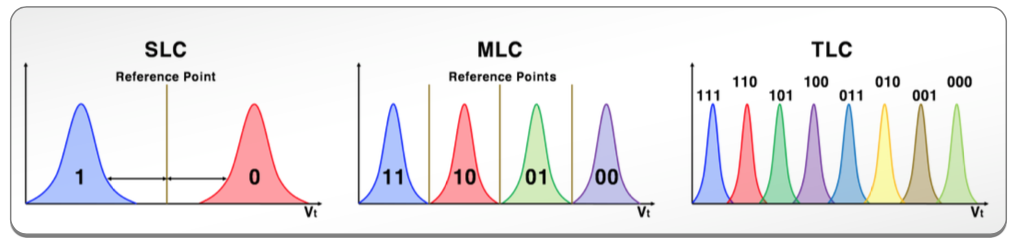
\includegraphics[width=0.5\textwidth]{img/img14.png}
    \caption{SSD}
    \label{fig:SSDs}
    \end{center}
\end{figure}
\end{multicols}
\subsubsection{Internal Organization}
NAND flash is organized into Pages and Blocks:\\
A {\bf page} contains multiple logical block (e.g. 512B-4KB) addresses (LBAs), a {\bf block} typically consists of multiple pages (e.g., 64) with a total capacity of around 128-256KB; Block/Page terminology in the SSD context can clash with previous use.\\
{\bf Blocks} (or Erase Block): smallest unit that can be erased. It consists of multiple pages and can be cleaned using the ERASE command.\\
{\bf Pages} : smallest unit that can be read/written. It is a sub-unit of an erase block and consists of the number of bytes which can be read/written in a single operations through the READ or PROGRAM commands.\\
Pages can be in three states:
\begin{itemize}
    \item Dirty (or INVALID): they contain data, but this data is no longer in use (or never used)
    \item Empty (or EREASED): they do not contain data
    \item In use (or VALID): the page contains data that can be actually read
\end{itemize}
Only empty pages can be written\\
Only dirty pages can be erased, but this must be done at the block
level (all the pages in the block must be dirty or empty)\\
It is meaningful to read only pages in the “in use” (“valid”) state\\
If no empty page exists, some dirty page must be erased:
\begin{itemize}
    \item If no block containing just dirty or empty pages exists, then special procedures should be followed to gather empty pages over the disk
    \item To erase the value in flash memory the original voltage must be reset to neutral before a new voltage can be applied, known as write amplification
\end{itemize}
{\bf Remark: we can write and read a single page of data from a SSD but we have to delete an entire block to release it}\\
\newline
{\bf WRITE AMPLIFICATION}: the actual amount of information physically written to the storage media is a multiple of the logical amount intended to be written.\\
\newline
{\bf Wear out}: breakdown of the oxide layer within the floating-gate transistors of NAND flash memory.\\
The erasing process hits the flash cell with a relatively large charge of electrical energy.\\
Each time a block is erased:
\begin{itemize}
    \item the large electrical charge actually degrades the silicon material
    \item after enough write-erase cycles, the electrical properties of the flash cell begin to break down and the cell becomes unreliable
\end{itemize}
{\bf Flash Translation Layer} = layer that matches the file system and the SSD.\\
\begin{multicols}{2}
\begin{figure}[H]
    \begin{center}
    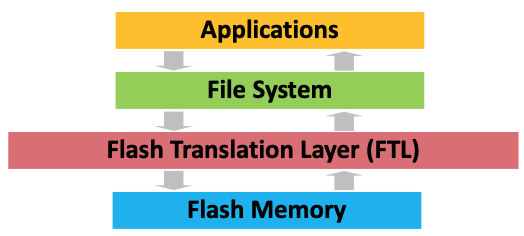
\includegraphics[width=0.5\textwidth]{img/img15.png}
    \caption{Flash Translation Layer}
    \label{fig:FTL}
    \end{center}
\end{figure}
\columnbreak
Direct mapping between Logical to Physical pages is not feasible\\
FTL is an SSD component that make the SSD “look as HDD”:
\begin{enumerate}
    \item Data Allocation and Address translation
    \begin{itemize}
        \item Efficient to reduce Write Amplification effects
        \item Program pages within an erased block in order (from low to high pages): Log-Structured FTL
    \end{itemize}
    \item Garbage collection: Reuse of pages with old data (Dirty/Invalid)
    \item  Wear leveling: FTL should try to spread writes across the blocks of the flash ensuring that all of the blocks of the device wear out at roughly the same time
\end{enumerate}
\end{multicols}

{\bf Garbage collection}\\
When an existing page is updated à old data becomes obsolete!\\
Old version of data are called garbage and (sooner or later) garbage pages must be reclaimed for new writes to take place.\\
Garbage Collection is the process of finding garbage blocks and reclaiming them: Simple process for fully garbage blocks or more complex for partial cases. I.e. Basic steps: 
\begin{enumerate}
    \item Find a suitable partial block
    \item Copy non-garbage pages
    \item Reclaim (erase) the entire block for writing
\end{enumerate}
\begin{figure}[H]
    \begin{center}
    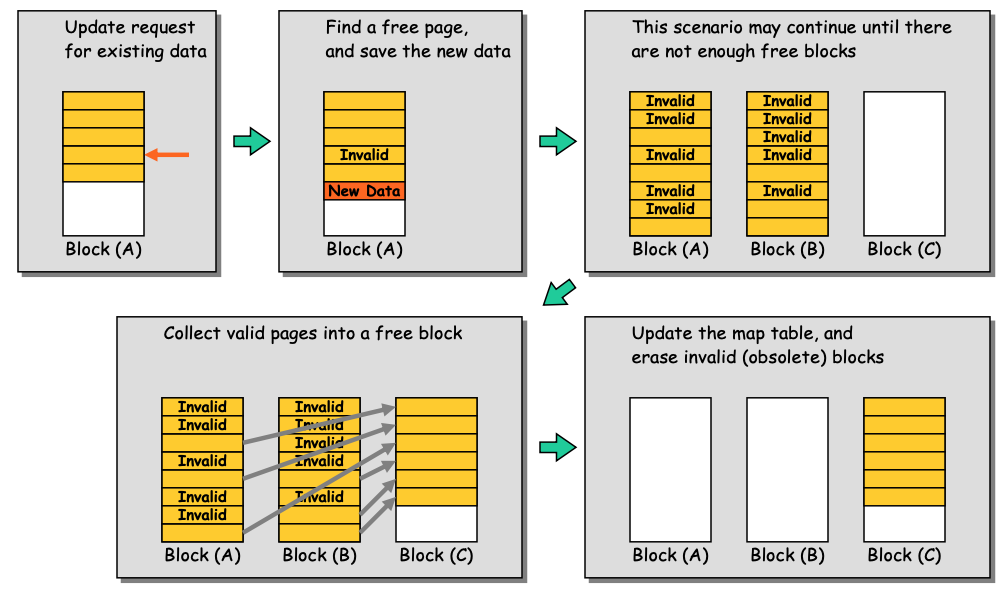
\includegraphics[width=0.4\textwidth]{img/img16.png}
    \caption{Garbage collection (Example)}
    \label{fig:GC ex}
    \end{center}
\end{figure}
Garbage collection is expensive: Require reading and rewriting of live data and the ideal garbage collection is reclamation of a block that consists of only dead pages.\\
The {\bf8cost} of Garbage Collection depends on the amount of data blocks that have to be migrated.\\
Solutions to alleviate the problem:
\begin{itemize}
    \item Overprovision the device by adding extra flash capacity: Cleaning can be delayed
    \item Run the Garbage Collection in the background using less busy periods for the disk
\end{itemize}
When performing background GC the SSD assumes to know which pages are invalid\\
{\bf Problem}: most file systems don’t actually delete data (E.g., on Linux, the “delete” function is unlink() and it removes the file meta-data, but not the file itself)
\begin{figure}[H]
    \begin{center}
    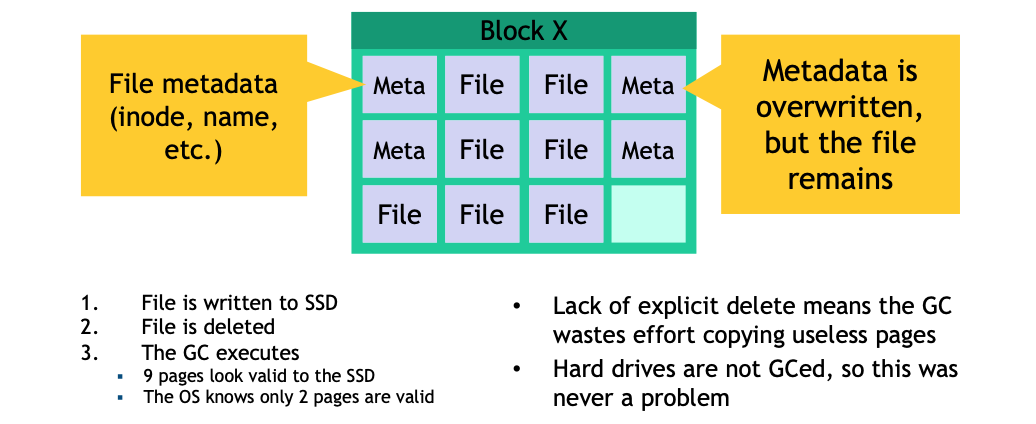
\includegraphics[width=0.8\textwidth]{img/img17.png}
    \caption{Garbage collection (Example)}
    \label{fig:GC ex}
    \end{center}
\end{figure}
New SATA command TRIM (SCSI – UNMAP): The OS tells the SSD that specific LBAs are invalid and may be GCed.\\
OS support for TRIM (Win 7, OSX Snow Leopard, Linux 2.6.33, Android 4.3).\\
\newline
The size of page-level mapping table is too large:
With a 1TB SSD with a 4byte entry per 4KB page, 1GB of is needed for mapping.\\
Some approaches to reduce the costs of mapping:
\begin{itemize}
    \item \underline{Block-based mapping}: Coarser grain approach.\\
    Mapping at block granularity, to reduce the size of a mapping table. Small write problem: the FTL must read a large amount of live data from the old block and copy them into a new one.
    \item \underline{Hybrid mapping} : Multiple tables.\\
    FTL maintains two tables:
    \begin{itemize}
        \item Log blocks: page mapped
        \item Data blocks: block-mapped
    \end{itemize}
    When looking for a particular logical block, the FTL will consult the page mapping table and block mapping table in order
    \item \underline{Page mapping plus caching} : Exploiting Data Locality.\\
    Basic idea is to cache the active part of the page-mapped FTL, f a given workload only accesses a small set of pages, the translations of those pages will be stored in the FTL memory. High performance without high memory cost if the cache can contain the necessary working set. Cache miss overhead. exists
\end{itemize}
{\bf Wear Leveling}\\
Erase/Write cycle is limited in Flash memory:\\
- Skewness in the EW cycles shortens the life of the SSD\\
- All blocks should wear out at roughly the same time\\
Log-Structured approach and garbage collection helps in spreading writes. However, a block may consist of cold data 
\begin{itemize}
    \item the FTL must periodically read all the live data out of such blocks and re-write it elsewhere
    \item Wear leveling increases the write amplification of the SSD and decreases performance (Simple Policy: Each Flash Block has EW cycle counter, Maintain |Max(EW cycle) – Min(EW cycle)|$<$ e)
\end{itemize}

\subsubsection{SSD summary}
\begin{itemize}
    \item They cost more than the conventional HDD
    \item Flash memory can be written only a limited number of times (wear):\\
    have a shorter lifetime\\
    error correcting codes\\
    over-provisioning (add some spare capacity)
    \item Different read/write speed\\
    Write amplification
    \item Write performance degrades of one order of magnitude after the first writing
    \item Often the controller become the real bottleneck to the transfer rate
    \item SSD are not affected by data-locality and must not be defragmented (actually, defragmentation may damage the disks)
    \item Flash Translation Layer is one of the key components\\
    - Data Allocation\\
    - Address Translation\\
    - Garbage Collection\\
    - Wear Leveling
\end{itemize}

\subsection{HDD vs SSD}
\begin{multicols}{2}
{\bf Unrecoverable Bit Error Ratio} (UBER): A metric for the rate of occurrence of data errors, equal to the number of data errors per bits read\\ 
{\bf Endurance rating} : Terabytes Written (TBW is the total amount of data that can be written into an SSD before it is likely to fail). The number of terabytes that may be written to the SSD while still meeting the requirements\\
\columnbreak
\begin{figure}[H]
    \begin{center}
    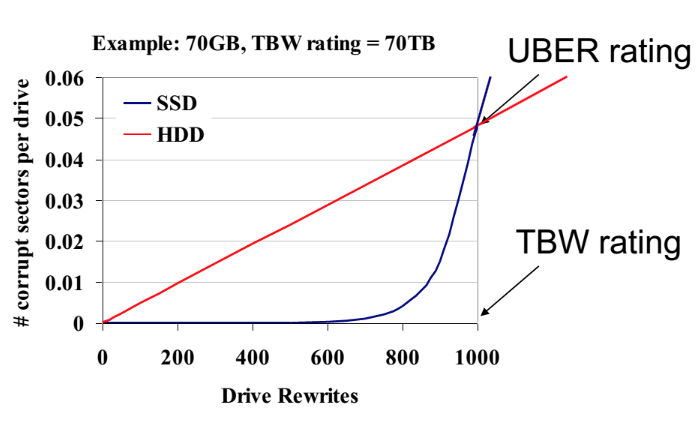
\includegraphics[width=0.3\textwidth]{img/img18.png}
    \caption{Garbage collection (Example)}
    \label{fig:GC ex}
    \end{center}
\end{figure}
\end{multicols}
Memory cells can accept data recording between 3,000 and 100,000 during its lifetime: once the limit value is exceeded, the cell "forgets" any new data\\
\newline
A typical TBW for a 250 GB SSD is between 60 and 150 Terabytes of data written to the drive; This means that in order to overcome, for example, a TBW of 70 Terabytes, a user should write 190 GB every day for a year or fill his SSD on a daily basis for two thirds with new files for a whole year\\
\newline
It is difficult to comment on the duration of SSDs: Dell, in an old study (2011), spoke of an estimated duration between three months and ten years explaining, however, that there are so many factors (temperature and workload) that may depend on the life of an SSD that is very difficult to make predictions.

\subsection{Hybrid solution}
HDD + SSD
\begin{itemize}
    \item Some large storage servers use SSD as a cache for several HDD. Some mainboards of the latest generation have the same feature: they combine a small SSD with a large HDD to have a faster disk.
    \item Some HDD manufacturers produce Solid State Hybrid Disks (SSHD) that combine a small SDD with a large HDD in a single unit.
\end{itemize}


\subsection{Storage system}
\begin{multicols}{2}
\begin{figure}[H]
    \begin{center}
    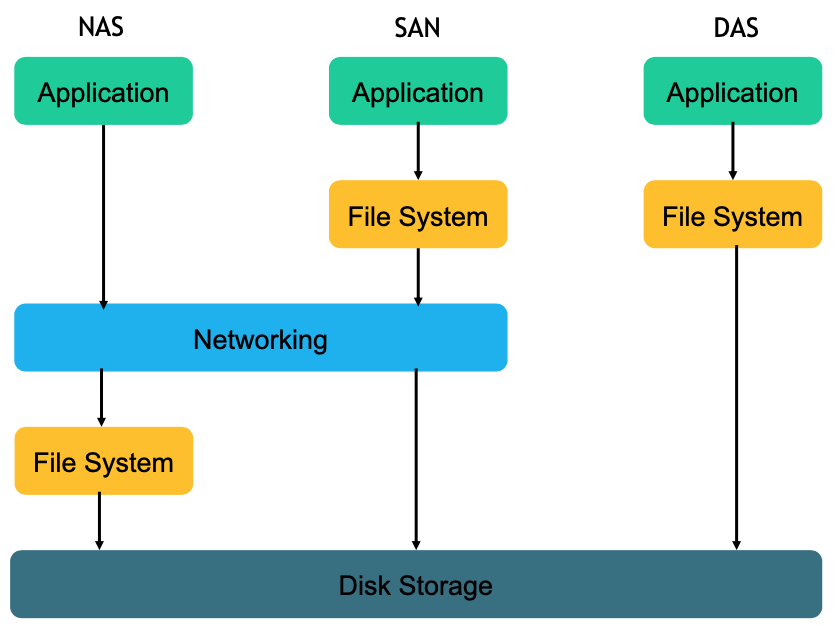
\includegraphics[width=0.4\textwidth]{img/img19.png}
    \caption{NAS SAN DAS}
    \label{fig:NAS SAN DAS}
    \end{center}
\end{figure}
\columnbreak
\begin{defn}
A {\bf Direct Attached Storage} (DAS) is a storage system directly attached to a server or workstation. They are visible as disks/volumes by the client OS.
\end{defn}
\begin{defn}
A {\bf Network Attached Storage} (NAS) is a computer connected to a network that provides only file-based data storage services (e.g., FTP, Network File System and SAMBA) to other devices on the network and is visible as File Server to the client OS
\end{defn}
\begin{defn}
{\bf Storage Area Networks} (SAN) are remote storage units that are connected to a server using a specific networking technology (e.g., Fiber Channel) and are visible as disks/volumes by the client OS
Direct Attached Storage (DAS) is a storage system directly
\end{defn}
\end{multicols}



\subsubsection{DAS}
DAS is a storage system directly attached to a server or workstation\\
The term is used to differentiate non-networked storage from SAN and NAS (that will be described later).\\
{\bf Main features}:
\begin{itemize}
    \item limited scalability (for ex. if I want 100 server connected, I have to multiply x100 the capacity)
    \item complex management
    \item to read files in other machines, the “file sharing” protocol of the OS must be used (on application laver, if I have one Windows and one Linux they must be able to communicate)
\end{itemize}
{\bf Internal and external}:
\begin{itemize}
    \item DAS does not necessary mean “internal drives” (it could have an external hard disk)
    \item All the external disks, connected with a point-to-point protocol to a PC can be considered as DAS
\end{itemize}

\subsubsection{NAS}
A NAS unit is a computer connected to a network that provides only file-based data storage services to other devices on the network.\\
NAS systems contain one or more hard disks, often organized into logical redundant storage containers or RAID.\\
Provide file-access services to the hosts connected to a TCP/IP network though Networked File Systems/SAMBA.\\
Each NAS element has its own IP address.\\
Good scalability (incrementing the devices in each NAS element
or incrementing the number of NAS elements).\\
\newline
{\bf NAS vs DAS}\\
The key differences between direct-attached storage (DAS) and NAS are:
\begin{itemize}
    \item DAS is simply an extension of an existing server and is not necessarily networked
    \item NAS is designed as an easy and self-contained solution for sharing files over the network
\end{itemize}
Comparing NAS with local (non-networked) DAS, the {\sl performance} of NAS depends mainly on the speed of and congestion on the network

\subsubsection{SAN}
Storage Area Networks, are remote storage units that are connected to a PC/server using a specific networking technology.\\
SANs have a special network devoted to the accesses to storage devices.\\
Two distinct networks (one TCP/IP and one dedicated network, e.g., Fber Channer).\\
High scalability (simply increasing the storage devices connected to the SAN network).\\
\newline
{\bf NAS vs SAN}\\
\begin{itemize}
    \item NAS provides both storage and a file system
    \item This is often contrasted with SAN which provides only block-based storage and leaves file system concerns on the "client" side
    \item One way to loosely conceptualize the difference between a NAS and a SAN is that:
    \begin{itemize}
        \item NAS appears to the client OS (operating system) as a file server (the client can map network drives to shares on that server)
        \item a disk available through a SAN still appears to the client OS as a disk: it will be visible in the disks and volumes management utilities (along with client's local disks), and available to be formatted with a file system
    \end{itemize}
    \item NAS is used for low-volume access to a large amount of storage by many users
    \item SAN is the solution for petabytes (1012) of storage and multiple, simultaneous access to files, such as streaming audio/video
\end{itemize}

\begin{figure}[H]
    \begin{center}
    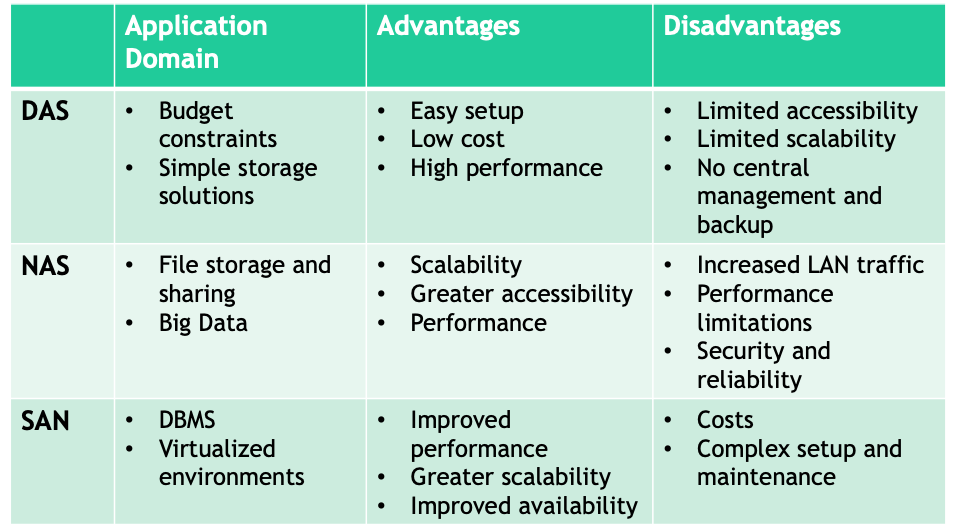
\includegraphics[width=0.5\textwidth]{img/img20.png}
    \caption{NAS vs SAN vs DAS}
    \label{fig:NAS,SAN,DAS}
    \end{center}
\end{figure}

\newpage

%------------------------------------------------------%
\section{Networking}
{\sl Communication} equipment allows network interconnections among the devices.\\
They can be:
\begin{itemize}
    \item Hubs
    \item Routers
    \item DNS or DHCP servers
    \item Load balancers
    \item Technology switches
    \item Firewalls
\end{itemize}
The performance of servers increases over time, the demand for inter-server bandwidth naturally increases as well!\\
{\sl We can double the aggregate compute capacity or the aggregate storage simply by doubling the number of compute or storage elements}, but how?\\
Networking has no straightforward horizontal scaling solution.\\
Doubling leaf bandwidth is easy: with twice as many servers, we’ll have twice as many network ports and thus twice as much bandwidth.
\begin{multicols}{2}
\noindent
But if we assume that every server needs to talk to every other server, we need to deal with {\bf bisection bandwidth}. \begin{defn}The bandwidth across the narrowest line that equally divides the cluster into two parts. Characterizes network capacity since randomly communicating processors must send data across the “middle” of the network
\end{defn}
\columnbreak
\begin{figure}[H]
    \begin{center}
    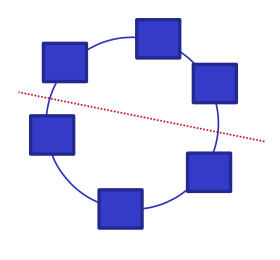
\includegraphics[width=0.2\textwidth]{img/img21.png}
    \caption{bisection bandwidth}
    \label{fig:bisection bandwidth}
    \end{center}
\end{figure}
\end{multicols}
\subsection{Architecture}
\begin{figure}[H]
    \begin{center}
    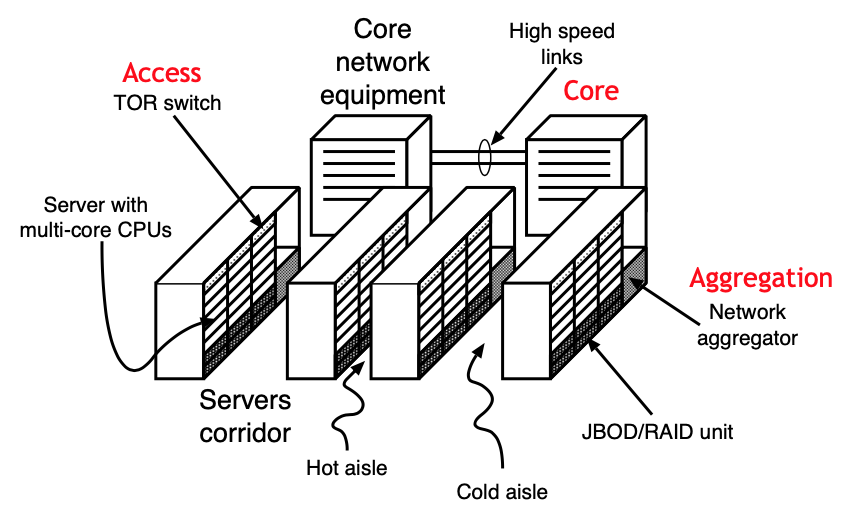
\includegraphics[width=0.4\textwidth]{img/img22.png}
    \caption{Data-center network architectures}
    \label{fig:DS net architecture}
    \end{center}
\end{figure}
Switches at the access layer can be put into two positions:
\begin{itemize}
    \item {\sl Top-Of-the-Rack} (TOR): {\bf Access} switches are put at the top of each rack. The number of cables is limited. The number of ports per switch is also limited (lower costs). However, the scalability is also limited.
    \item {\sl End-Of-the-Line} (EOL): Switches are positioned one per corridor, at the end of a line of rack. {\bf Aggregation} switches must have a larger number of ports, and longer cables are required (higher costs). However, the system can scale to have a larger number of machines.
\end{itemize}
Three layer architecture configures the network in three different
layers:
\begin{itemize}
    \item core
    \item aggregation
    \item access
\end{itemize}
{\bf Bandwidth} can be increased by increasing the switches at the core and aggregation layers, and by using routing protocols such as Equal Cost Multiple Path (ECMP) that equally shares the traffic among different routes.\\
\newline
This solution is very simple, but can be very expensive in large data-centers since:\\
• Upper layers require faster network equipments. (For example: 1 GB Ethernet at the access layer, 10 GB Ethernet at the aggregation layer, 25 GB Optical connections at the core layer)\\
• The cost in term of acquisition and energy consumption can be very high\\
{\sl Another benefit of SANs: a way to tackle network scalability, offload some traffic to a special-purpose network connecting servers to storage units
}
\begin{multicols}{2}
    \begin{figure}[H]
        \begin{center}
        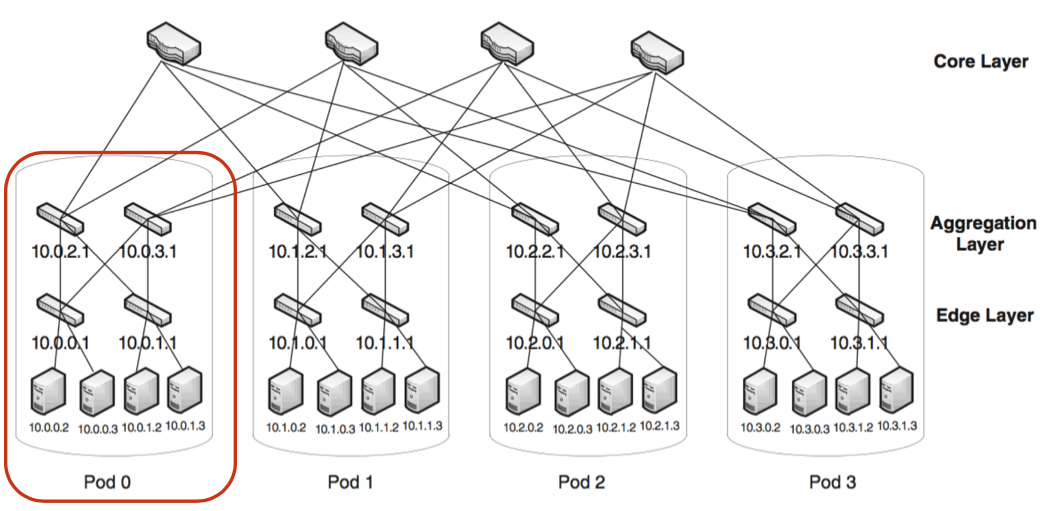
\includegraphics[width=0.3\textwidth]{img/img23.png}
        \caption{Fat-tree topologies}
        \label{fig:Fat-tree topologies}
        \end{center}
    \end{figure}
Fat-tree topologies use a larger number of slower speed switches and connections. In particular, nodes are divided into pods characterized by the same number of nodes and switches.
    \columnbreak
    \begin{figure}[H]
        \begin{center}
        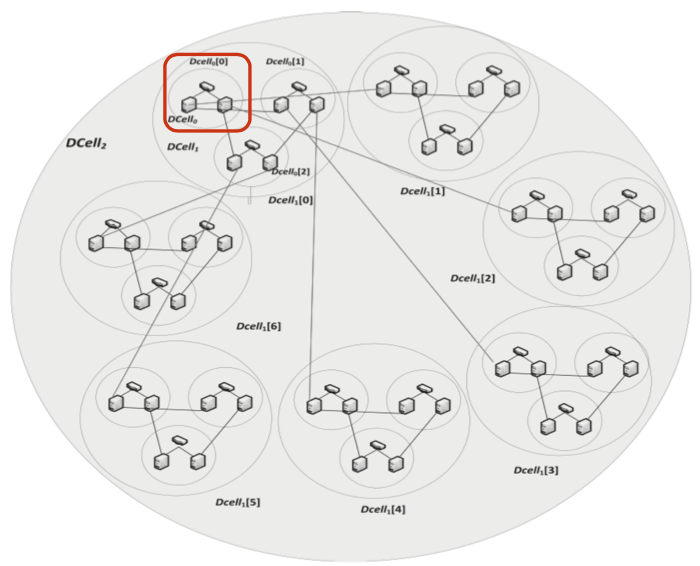
\includegraphics[width=0.2\textwidth]{img/img24.png}
        \caption{D-Cell topology}
        \label{fig:D-Cell topology}
        \end{center}
    \end{figure}
D-Cell topology, defines the network in recursive way. Cells are organized in levels. Switches connects nodes at the lower level.Some nodes belong to different cells: they perform routing among them to create a higher level cell. 
\end{multicols}
\subsubsection{High Performance Clusters}
High-Performance Computing (HPC) supercomputer clusters often have a much lower ratio of computation to network bandwidth.\\
\newline
Applications (e.g., weather simulations) distribute their data across RAM in all nodes, and nodes need to update neighboring nodes after performing relatively few floating-point computations.\\
Traditional HPC systems have used proprietary interconnects with leading-edge link bandwidths, much lower latencies, and some form of a global address space (where the network is integrated with CPU caches and virtual addresses)\\
\newline
High {\bf throughputs} but much more expensive solutions.
\subsection{Network to support Virtualization}
Connection endpoints (i.e., IP address/port combinations) can move from one physical machine to another\\ 
Typical networking hardware as well as network management software don’t anticipate such moves and in fact often explicitly assume that they’re not possible \\ (All machines in a given rack have IP addresses in a common subnet, which simplifies administration and minimizes the number of required forwarding table entries routing tables)\\ \underline{Solution}: the cluster manager that decides the placement of computations also updates the network state through programmable Network control planes (Software Defined Networks)
\subsection{The interplay of storage and networking technology}
The success of WSC distributed storage systems can be partially attributed to the evolution of data center networking fabrics:{\sl disk locality is no longer relevant in intra-data center computations}.\\
This observation enables:
\begin{itemize}
    \item simplifications in the design of distributed disk-based storage
    systems
    \item utilization improvements
\end{itemize}since any disk byte in a WSC facility can, in principle, be utilized by any task regardless of their relative locality
\subsection{Balanced design}
{\sl  Computer architects are trained to solve the problem of finding the right combination of performance and capacity from the various building blocks that make up a WSC}\\ \\
The right building blocks are apparent only when one considers the entire WSC system.\\
It is important to characterize the kinds of workloads that will execute on the system with respect to their consumption of various resources.\\
Keeping in mind three important considerations:
\begin{enumerate}
    \item Smart programmers may be able to restructure their algorithms to
    better match a more inexpensive design alternative
    \item The most cost-efficient and balanced configuration for the hardware may be a match with the combined resource requirements of multiple workloads
    \item Fungible resources tend to be more efficiently used
\end{enumerate}
System balance: {\bf Storage Hierarchy}
\subsubsection*{Example}
\begin{multicols}{2}
We assume a system with 5,000 servers, each with 256 GB of DRAM, one 4 TB SSD, and eight 10 TB disk drives.\\
Each group of 40 servers is connected through a 40-Gbps link to a rack-level switch (TOR)\\
Each rack has an additional 10-Gbps uplink bandwidth per machine for connecting the rack to the cluster-level switch (AGGREGATION)\\
Network latency numbers assume a TCP/IP transport, and networking bandwidth values assume that each server is using its fair share of the available cluster-level bandwidth.\\
For disks, typical commodity disk drive (SA T A) latencies and transfer rates are considered.
\columnbreak
\begin{figure}[H]
    \begin{center}
    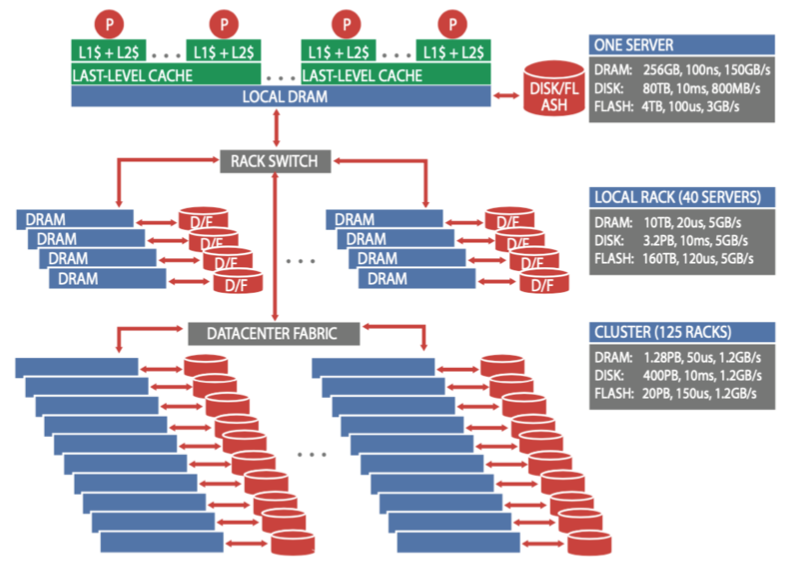
\includegraphics[width=0.4\textwidth]{img/img25.png}
    \caption{Storage Hierarchy}
    \label{fig:Storage Hierarchy}
    \end{center}
\end{figure}
\end{multicols}
A large application that requires servers in many racks to operate must deal effectively with large discrepancies in latency, bandwidth, and capacity.\\
\newline
These discrepancies are much larger than those seen on a single machine, making it more difficult to program a WSC:
\begin{itemize}
    \item A key challenge for architects of WSCs is to smooth out these discrepancies in a cost-efficient manner
    \item A key challenge for software architects is to build SW infrastructure and services that hide this complexity
\end{itemize} Three specific comments about SSDs:
\begin{enumerate}
    \item Much faster than HDDs
    \item Demand a high bandwidth
    \item In the worst case, writes to flash can be several orders of magnitude slower than reads
\end{enumerate}

\newpage
%------------------------------------------------------%

\section{Building and Infrastructures}
\begin{figure}[H]
    \begin{center}
    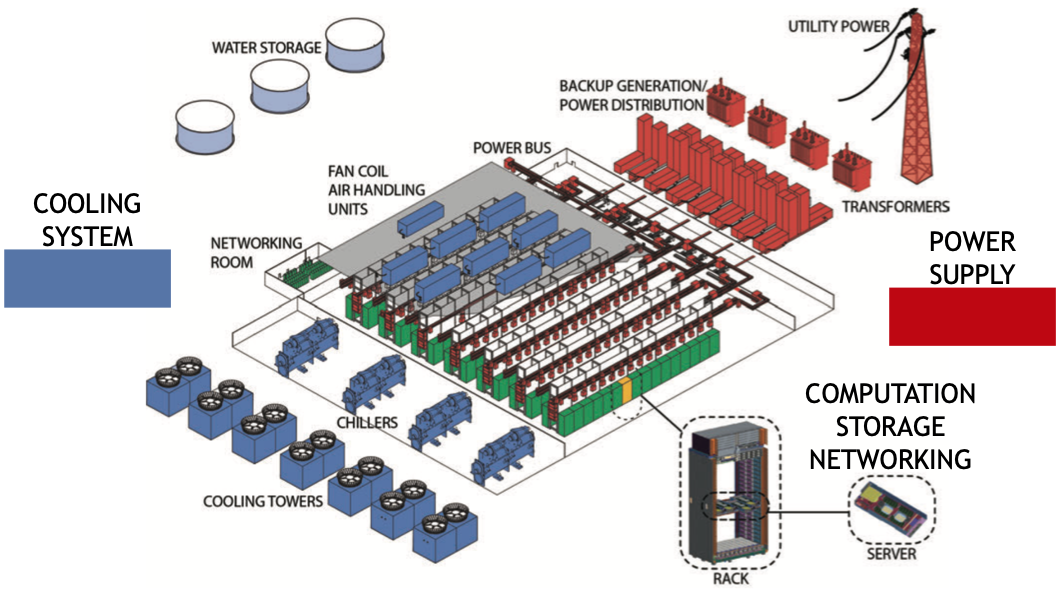
\includegraphics[width=0.7\textwidth]{img/img26.png}
    \caption{Main components of a typical data center}
    \label{fig:Main components}
    \end{center}
\end{figure}
WSC has not just computation, storage and networking; it has other important components related to power delivery, cooling, and building infrastructure that also need to be considered.
\subsection{Power System}
In order to protect against power failure, battery and diesel generators are used to backup the external supply.\\ \\
The UPS typically combines three functions in one system:
\begin{enumerate}
    \item contains a transfer switch that chooses the active power input (either utility power or generator power)
    \item contains some form of energy storage (electrical, chemical, or mechanical) to bridge the time between the utility failure and the availability of generator power
    \item conditions the incoming power feed, removing voltage spikes or sags, or harmonic distortions in the AC feed
\end{enumerate}
\subsection{Cooling System}
IT equipment generates a lot of heat: the cooling system is usually a very expensive component of the datacenter, and it is composed by coolers, heat-exchangers and cold water tanks.
\subsubsection{Open-Loop}
The simplest topology is fresh air cooling (or air economization)— essentially, opening the windows. This is a single «open-loop» system.
\begin{defn}
    Free cooling, i.e., open-loop, refers to the use of cold outside air to either help the production of chilled water or directly cool servers. It is not completely free in the sense of zero cost, but it involves very low-energy costs compared to chillers. 
\end{defn}
\subsubsection{Closed-Loop}
\begin{defn}
    Closed-loop systems come in many forms, the most common being the air circuit on the data center floor.
\end{defn}
The goal is to isolate and remove heat from the servers and transport it to a heat exchanger.\\ Cold air flows to the servers, heats up, and eventually reaches a heat exchanger to cool it down again for the next cycle through the servers.
\begin{multicols}{2}
\begin{figure}[H]
    \begin{center}
    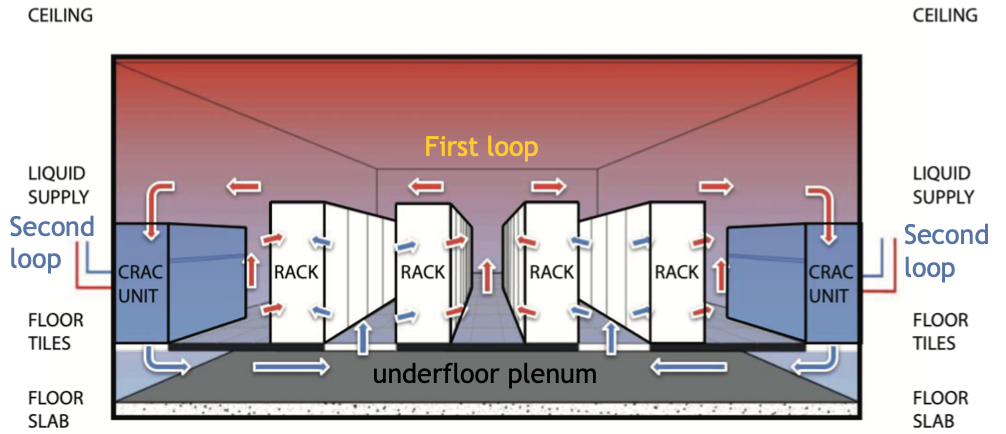
\includegraphics[width=0.5\textwidth]{img/img27.png}
    \caption{Closed-loop with two loop}
    \label{fig:Closed-loop with two loop}
    \end{center}
\end{figure}
\columnbreak
\subsubsection*{Closed-loop with two loops}
\begin{itemize}
    \item The airflow through the underfloor plenum, the racks, and back to the CRAC (a 1960s term for computer room air conditioning) defines the primary air circuit, i.e., the {\bf first loop}.
    \item The {\bf second loop} (the liquid supply inside the CRACs units) leads directly from the CRAC to external heat exchangers (typically placed on the building roof) that discharge the heat to the environment.
\end{itemize}
\end{multicols}
\subsubsection*{A three-loop system commonly used in large-scale data center}
\begin{figure}[H]
    \begin{center}
    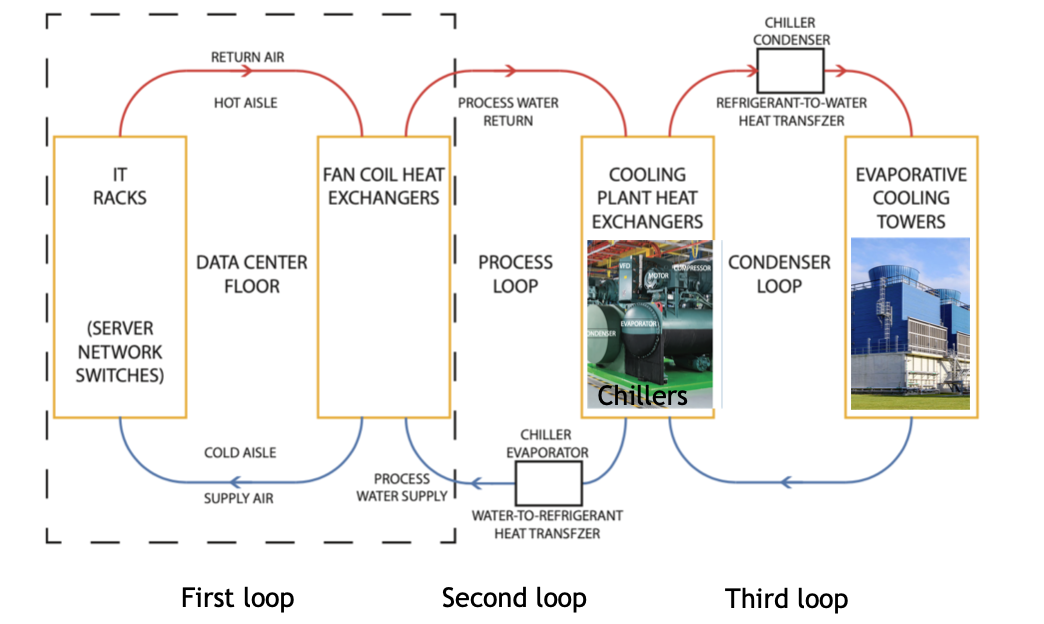
\includegraphics[width=0.4\textwidth]{img/img28.png}
    \caption{Closed-loop with three loop}
    \label{fig:Closed-loop with three loop}
    \end{center}
\end{figure}
A water-cooled {\bf chiller} can be thought of as a water-cooled air conditioner.\\
\newline
{\bf Cooling towers} cool a water stream by evaporating a portion of it into the atmosphere. They do not work as well in very cold climates because they need additional mechanisms to prevent ice formation
\subsubsection{Comparison}
Each topology presents tradeoffs in complexity, efficiency, and cost:
\begin{itemize}
    \item Fresh air cooling can be very efficient but does not work in all climates, requires filtering of airborne particulates, and can introduce complex control problems.
    \item Two-loop systems are easy to implement, relatively inexpensive to construct, and offer isolation from external contamination, but typically have lower operational efficiency.
    \item A three-loop system is the most expensive to construct and has moderately complex controls, but offers contaminant protection and good efficiency.
\end{itemize}
\subsubsection{In-rack cooling}
In-rack cooler adds an air-to-water heat exchanger at the back of a rack so the hot air exiting the servers immediately flows over coils cooled by water, essentially reducing the path between server exhaust and CRAC input
\subsubsection{In-row cooling}
In-row cooling works like in-rack cooling except the cooling coils are not in the rack, but adjacent to the rack.
\subsubsection{Liquid cooling}
We can directly cool server components using \underline{cold plates}, i.e., local liquid-cooled heat sinks:
\begin{itemize}
    \item Impractical to cool all compute components with cold plates.
    \item Components with the highest power dissipation are targeted
    for liquid cooling while other components are air-cooled.
\end{itemize}
The liquid circulating through the heat sinks transports the heat to a liquid-to-air or liquid-to-liquid heat exchanger that can be placed close to the tray or rack, or be part of the data center building (such as a cooling tower).
\subsubsection*{Container-based}
Container-based data centers go one step beyond in-row cooling by placing the server racks inside a container (typically 6 to 12 mt long) and integrating heat exchange and power distribution into the container as well.

\subsection{Power consumption}
Data-center power consumption is an issue, since it can reach several MWs.\\
Cooling usually requires about half the energy required by the IT equipment (servers + network + disks).\\
Energy transformation creates also a large amount of energy wasted for running a datacenter.\\
\begin{itemize}
    \item DCs consume 3\% of global electricity supply (416.2 TWh > UK’s 300 TWh).
    \item DCs produce 2\% of total greenhouse gas emissions (same as worldwide air traffic pre-pandemic).
    \item DCs produce as much CO2 as The Netherlands or Argentina.
\end{itemize}
\begin{figure}[H]
    \begin{center}
    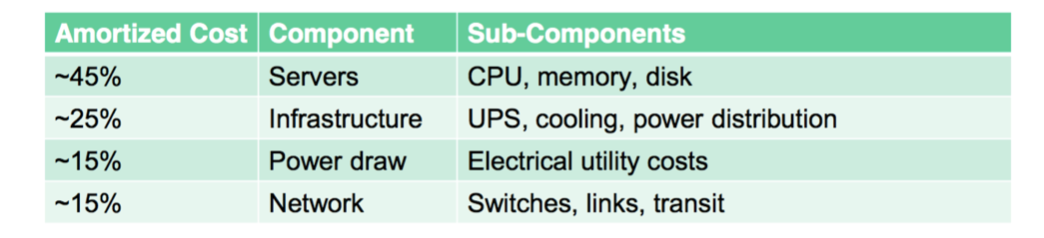
\includegraphics[width=0.6\textwidth]{img/img29.png}
    \caption{power consumption}
    \label{fig:power consumption}
    \end{center}
\end{figure}
\begin{defn}
    {\bf Power usage effectiveness} (PUE) is the ratio of the total amount of energy used by a DC facility to the energy delivered to the computing equipment
\end{defn}
PUE = $\frac{Total Facility Power}{IT Equipment power}$ 
\newline\newline
{\bf Total facility power} = covers IT systems (servers, network, storage) + other equipment (cooling, UPS, switch gear, generators, lights, fans, etc.)\\
{\bf Data Center infrastructure Efficiency} (DCiE): PUE inverse
\newline\newline

\subsection{Tiers}
Data-center availability is defined by in four different tier level. Each one has its own requirements.
\begin{figure}[H]
    \begin{center}
    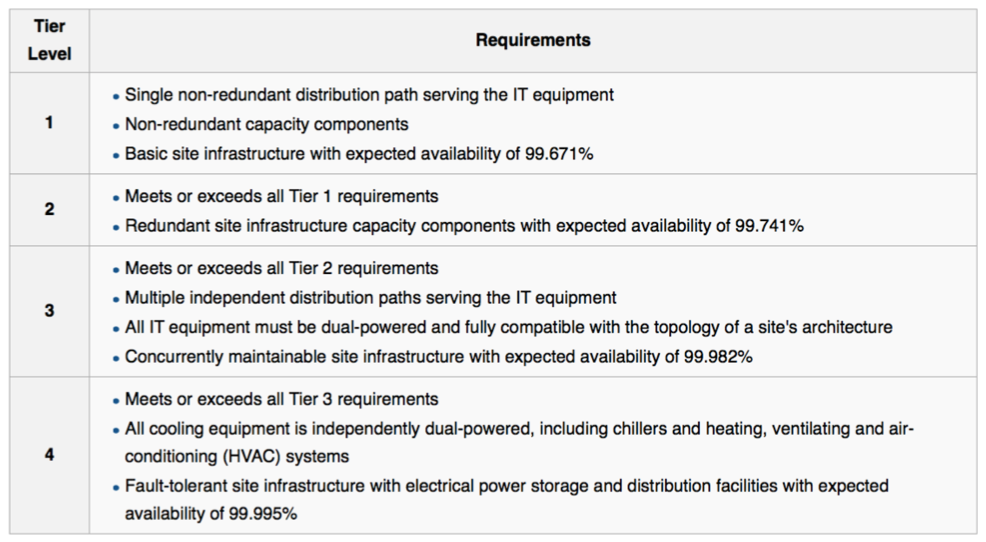
\includegraphics[width=0.6\textwidth]{img/img30.png}
    \caption{data-center tiers}
    \label{fig:tiers}
    \end{center}
\end{figure}

\newpage
%------------------------------------------------------------------%

\section{Virtualization}
\subsection{Cloud Computing}
\begin{defn}
    A coherent, large-scale, publicly accessible collection of computing, storage, and networking resources. Available via Web service calls through the Internet. Short- or long-term access on a pay-per-use basis
\end{defn}
\subsection*{How is Cloud implemented? Virtualization}
Hardware resources (CPU, RAM, ecc...) are partitioned and shared among multiple {\sl virtual machines} (VMs).\\
The {\sl virtual machine monitor} (VMM) governs the access to the physical resources among running VMs.\\
In this way are provided performance, isolation and security.
\subsection{Virtual Machines}
\begin{defn}
    A {\bf Machine} is an execution environment capable of running a program.
\end{defn}
\subsection*{What’s the difference between a physical machine and a virtual machine?}
Start from the {\bf computer architecture}: 
\begin{itemize}
    \item Sets of instructions characterized by
    the levels at which are considered
    \item OS creates new instructions for programs to access devices/hw
    \item the set of instructions that a program can use might be structured at different levels\\ (We usually program the software part, exploiting the hardware.)
\end{itemize}
\begin{multicols}{2}
    \begin{figure}[H]
        \begin{center}
        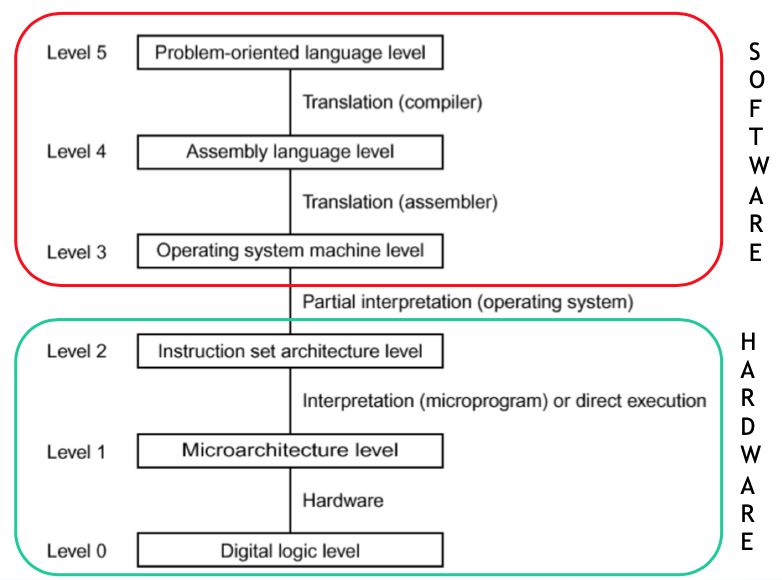
\includegraphics[width=0.5\textwidth]{img/img31.png}
        \caption{machine levels}
        \label{fig:machine levels}
        \end{center}
    \end{figure}
    \columnbreak
The ISA (Instruction Set Architecture) corresponds to {\bf Level 2} in the layered execution model. \\ISA marks the division between hardware and software.
    \begin{itemize}
        \item \underline{User ISA}: aspects of the ISA that are visible to an application program (sum, multiplication,..., logical operations, branches, etc...). When application interacts with the HW, User ISA is used.
        \item \underline{System ISA}: aspects visible to supervisor software (i.e., the OS) which is responsible for managing hardware resources (e.g., hide the complexity of CPUs, define how app access memory, communicate with the HW). When the OS interacts with the HW (Drivers, MM, Sched.), System ISA is used.
    \end{itemize}
The ABI (Application binary interface) corresponds to {\bf Level 3} in the layered execution model.\\ Provides a program (via the OS): the hardware resources and services available in a
system.
    \begin{itemize}
        \item \underline{User ISA}: aspects of the ISA that are visible to an application program (sum, multiplication,..., logical operations, branches, etc...).
        \item \underline{System Calls}: calls that allow programs to interact with shared hardware resources indirectly by OS
    \end{itemize}
\end{multicols}
\begin{defn}
    A {\bf Virtual Machine} (VM) is a logical abstraction able to provide a virtualized
execution environment. 
\end{defn}
More specifically, a VM:
\begin{itemize}
    \item (provides) Identical Software behavior
    \item (consists in a) Combination of physical machine and virtualizing software
    \item (may appear as) Different resources than physical machine
    \item (may result in) Different level of performance
\end{itemize}
Its {\bf tasks} are:\\
• To map virtual resources or states to corresponding physical ones\\
• To use physical machine instructions/calls to execute the virtual ones.\\ \\
Two {\bf types} of Virtual Machines:
\begin{enumerate}
    \item System VMs
    \item Process VMs
\end{enumerate}
\subsubsection{System VMs}
The VMM supports the levels 0-2 of the architecture.\\ \\
Provide a {\sl complete system environment} that can support an operating system (potentially with many user processes)\\
It provides {\sl operating system} running in it access to underlying hardware resources (networking, I/O, a GUI).\\ \\
The VM supports the operating system as long as the system environment is alive.\\
Virtualizing software placed between hardware and software ({\bf emulates the ISA interface} seen by software)\\ \\
The virtualization software is called VMM ({\bf Virtual Machine Monitor})\\\\
The VMM can provide its functionality either working {\bf directly} on the hardware, or running {\bf on another OS}.
\begin{figure}[H]
    \begin{center}
    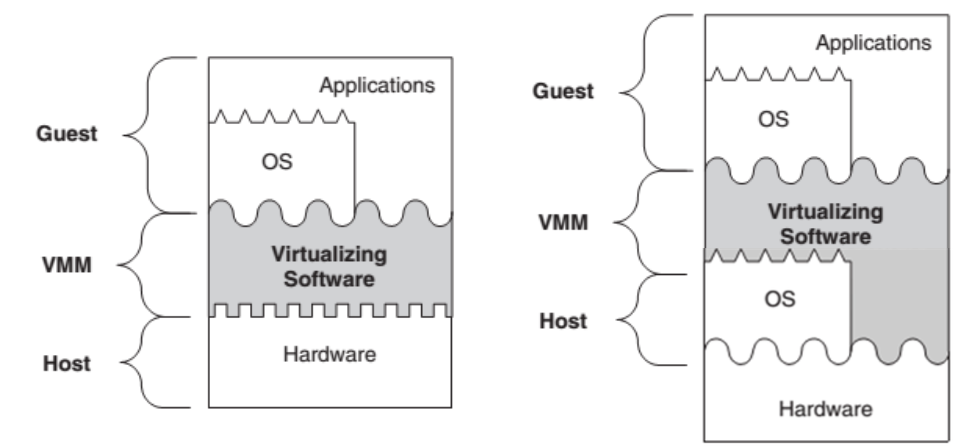
\includegraphics[width=0.5\textwidth]{img/img32.png}
    \caption{System Virtual Machine}
    \label{fig:System VMs}
    \end{center}
\end{figure}
\subsubsection{Process VMs}
The runtime software supports the levels 0-3 of the architecture
\begin{multicols}{2}
    \begin{figure}[H]
        \begin{center}
        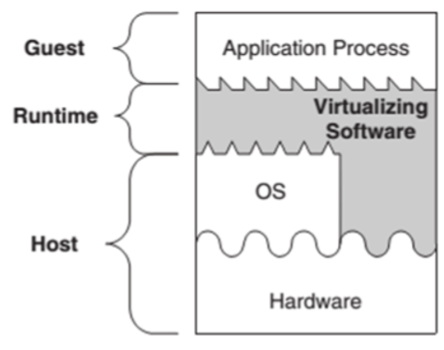
\includegraphics[width=0.3\textwidth]{img/img33.png}
        \caption{Process Virtual Machine}
        \label{fig:Process VMs}
        \end{center}
    \end{figure}
    \columnbreak
    Able to support an individual process\\ The virtualizing software is placed at the ABI interface, on top of the OS/hardware combination.\\ The virtualizing software emulates both user-level instructions and operating system calls.\\ The virtualization software is usually called {\bf Runtime Software}.
\end{multicols}
\begin{defn}
    {\bf Host} the underlying platform supporting the environment/system
\end{defn}
\begin{defn}
    {\bf Guest} the software that runs in the VM environment as the guest.
\end{defn}
\subsubsection{Process and System VMs}
\begin{figure}[H]
    \begin{center}
    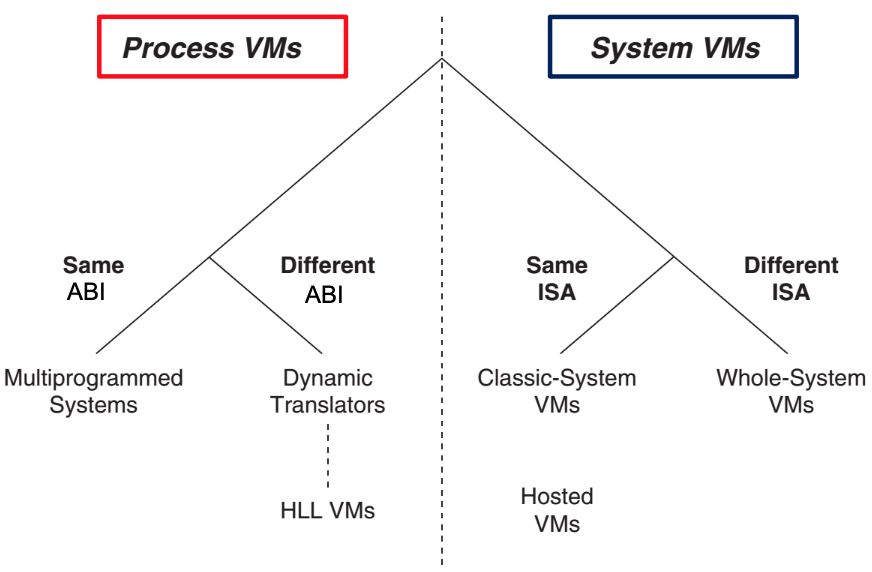
\includegraphics[width=0.5\textwidth]{img/img34.png}
    \caption{Different types of Virtualization}
    \label{fig:types of virtualization}
    \end{center}
\end{figure}
\subsubsection*{Multiprogrammed systems}
Same ABI / OS:\\
• VM formed by OS call interface + user ISA\\
• Common approach of all modern OS for multi user support (Task/Process Manager)\\
• Each user process is given:
\begin{itemize}
    \item the illusion of having a complete machine to itself.
    \item its own address space and is given access to a file structure
\end{itemize}
• OS timeshares and manages HW resources to permit this\\
• {\bf Arguable is a real VM}
\subsubsection*{Different ISA / ABI}
\begin{defn}
    {\bf Emulation} refers to those software technologies developed to allow an application (or OS) to run in an environment different from that originally intended.
\end{defn}It is required when the VMs have a different ISA / ABI from the architecture where they are running on.\\Example: Obsolete hardware emulators or other architectures emulators.\\\\
An {\bf emulator} reads all the bytes included in the memory of system it is going to reproduce.\\
Interpretation:
\begin{itemize}
    \item Interpreter program fetches, decodes, emulate the execution of individual source instruction
    \item Can be a slow process
    \item E.g., the Space Invaders (The system was based on the Intel 8080 CPU, with 8KB ROM, 1KB RAM, 7KB VRAM, plus a shift-register to speed up scrolling.)
\end{itemize}
\newpage
\subsubsection*{High-Level Language VM (HLL VMs)}
\begin{multicols}{2}
    \underline{Goal}: to have an isolated execution environment for each application (or for different instances of the same application).\\
    VM Task:
    \begin{itemize}
        \item Translates application byte code to OS-specific executable
        \item Minimize HW/OS-specific feature for platform independence
    \end{itemize}Applications run normally but: Sandboxed, Can “migrate”, Are not conflicting one another and Are not “installed” in a strict sense\\
Example: Java Virtual Machine (Java can work on every architecture for which an interpreter, called the Java Runtime Environment (JRE), exists)
    \columnbreak
    \noindent
    \begin{figure}[H]
        \begin{center}
        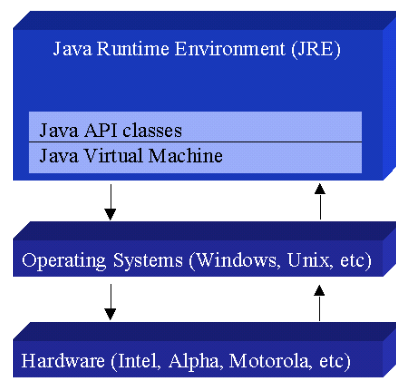
\includegraphics[width=0.3\textwidth]{img/img35.png}
        \caption{HLL VMs}
        \label{fig:HLL VMs}
        \end{center}
    \end{figure}
\end{multicols}
\subsubsection*{Same ISA}
\begin{multicols}{2}
    \begin{figure}[H]
        \begin{center}
        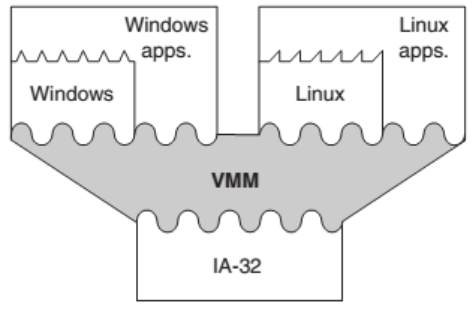
\includegraphics[width=0.2\textwidth]{img/img36.png}
        \caption{Classic system VMs}
        \label{fig:same ISA}
        \end{center}
    \end{figure}
    \columnbreak
    The VMM is on bare hardware, and virtual machines fit on top.\\
The VMM can intercept guest OS’s interaction with hardware resources.\\
The most efficient VM architecture (HW executes the same instructions of VMs)\\
Two different OSs on the same on the same HW
\end{multicols}

\subsubsection*{Hosted VM}
virtualizing software is on top of an existing host operating system.

\subsubsection*{Whole-system VMs}
\begin{multicols}{2}
    \begin{figure}[H]
        \begin{center}
        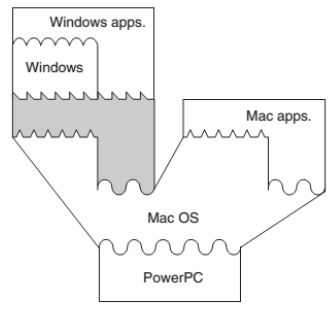
\includegraphics[width=0.2\textwidth]{img/img37.png}
        \caption{Whole system VMs}
        \label{fig:diff ISA}
        \end{center}
    \end{figure}
    \columnbreak
    Virtualize all software: ISAs are different so both application and OS code require emulation, e.g., via binary translation. (no native execution possible)\\Usually implement the VMM and guest software on top of a conventional host OS running on the hardware.\\the VM software must emulate the entire hardware environment and all the guest ISA operations to equivalent OS call to the Host.\\Example: MS Word and Windows running on a Power PC (not x86 family)
\end{multicols}

\subsection{Implementation}
Given a typical layered architecture of a system by {\sl adding layers} between execution stack layers.\\
Depending on where the new layer is placed, we obtain \underline{different types} of Virtualization.
\subsubsection{Hardware-level virtualization}Virtualization layer is placed between hardware and OS.\\The interface seen by OS and application might be different from the physical one
\subsubsection{Application-level virtualization}A virtualization layer is placed between
the OS and some applications (E.g.: JVM (Java Virtual Machine))\\Provides the same interface to the applications.\\Applications run in their environment, independently from OS
\subsubsection{System-level virtualization}The virtualization layer provides the interface of a physical machine to a secondary OS and a set of application running in it, allowing them to run on top of an existing OS.\\Placed between the system’s OS and other OS (E.g.: VMware Wks/Player, VirtualBox)\\Enable several OSs to run on a single HW

\subsection{Properties}
\begin{itemize}
    \item {\bf Partitioning}: \begin{itemize}
        \item Execution of multiple OSs on a single physical machine
        \item Partitioning of resources between the different VMs
    \end{itemize}
    \item {\bf Isolation}: \begin{itemize}
        \item Fault tolerance and security (as at the hardware level)
        \item Advanced resource control to guarantee performance
        (managed by the hypervisor)
    \end{itemize}
    \item {\bf Encapsulation}: \begin{itemize}
        \item The entire state of a VM can be saved in a file (e.g., freeze and restart the execution)
        \item Because a VM is a file, can be copied/moved as a file
    \end{itemize}
    \item {\bf HW-independence}: \begin{itemize}
        \item Provisioning/migration of a given VM on a given physical server .
    \end{itemize}
\end{itemize}

\subsection{Virtual Machine Manager (VMM)}
\begin{defn}
    An application that: \begin{itemize}
        \item manages the virtual machines
        \item mediates access to the hardware resources on the physical host
        system
        \item intercepts and handles any privileged or protected instructions
        issued by the virtual machines
    \end{itemize}
\end{defn}
This type of virtualization typically runs virtual machines whose operating system, libraries, and utilities have been compiled for the same type of processor and instruction set as the physical machine on which the virtual systems are running.
{\bf Crucial to support Cloud Computing}\\ \newline
Three terms are used to identify the same thing, some authors gives slightly different meanings:
\begin{itemize}
    \item {\sl Virtual Machine Monitor}: the virtualization software
    \item {\sl Hypervisor}: a virtualization software that runs directly on the hardware
    \item {\sl Virtual Machine Manager}: a VMM or Hypervisor that is also used to create, configure and maintain virtualized resources.
    It provides a user-friendly interface to the underlying virtualization software
\end{itemize}
\subsubsection*{Hyperversor types}
\begin{multicols}{4}
    \begin{figure}[H]
        \begin{center}
        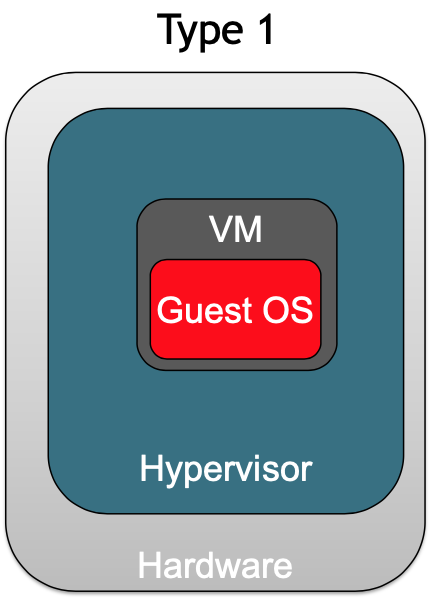
\includegraphics[width=0.15\textwidth]{img/img38.png}
        \caption{hyp type1}
        \label{fig:type1}
        \end{center}
    \end{figure}
    \columnbreak
    \noindent
    Bare-metal or type 1 hypervisors: akes direct control of the Hardware
    \columnbreak
    \begin{figure}[H]
        \begin{center}
        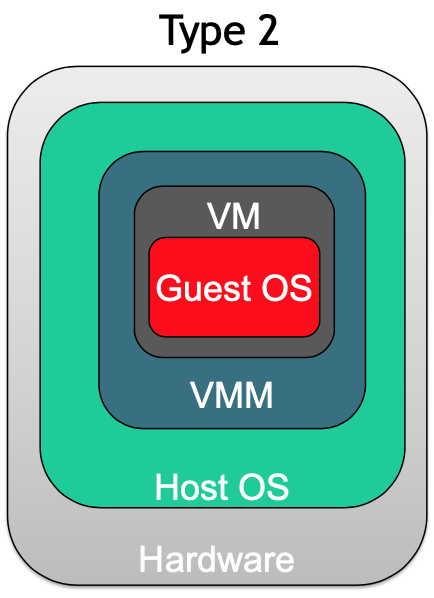
\includegraphics[width=0.15\textwidth]{img/img39.png}
        \caption{hyp type2}
        \label{fig:type2}
        \end{center}
    \end{figure}
    \columnbreak
    \noindent
    Hosted or type 2 hypervisors (VMM): reside within a host operating system and leverage code of the host OS (E.g. CPU scheduling, memory management)
\end{multicols}
\subsubsection{Type 1 hypervisor}
\begin{multicols}{4}
    \begin{figure}[H]
        \begin{center}
        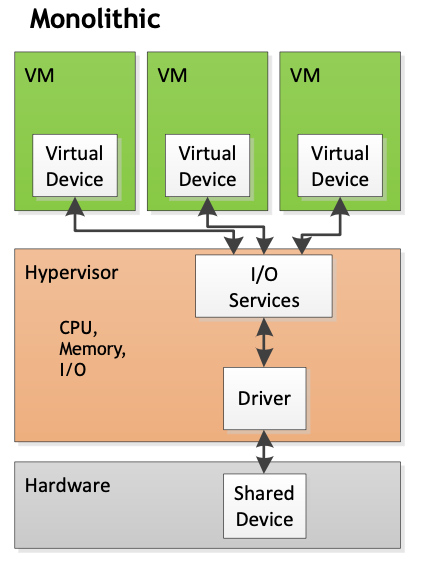
\includegraphics[width=0.2\textwidth]{img/img40.png}
        \caption{monolithic}
        \label{fig:monolithic}
        \end{center}
    \end{figure}
    \columnbreak
    \noindent
    Device drivers run within the hypervisor \begin{itemize}
        \item Better performance
        \item Better performance isolation
    \end{itemize}Can run only on hardware for which the hypervisor has drivers
    \columnbreak
    \begin{figure}[H]
        \begin{center}
        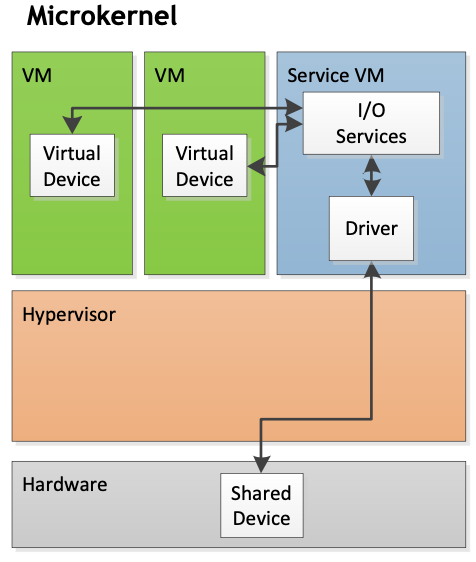
\includegraphics[width=0.2\textwidth]{img/img41.png}
        \caption{microkernel}
        \label{fig:Microkernel}
        \end{center}
    \end{figure}
    \columnbreak
    \noindent
    Device drivers run within a service VM \begin{itemize}
        \item Smaller hypervisor
        \item Leverages driver ecosystem of an existing OS
        \item Can use 3rd party driver (even if not always easy, recompiling might be required)
    \end{itemize}
\end{multicols}
\subsubsection*{Hacks}
Sometimes Type I Hypervisor can be used to provide hacks to some OSs.
Two well-known examples on PC hardware:\begin{enumerate}
    \item Windows 7 genuine without an official license: the Hypervisor mimics vendor specific hardware on different machines to allow the installation of pre-authorized S.O. copies (e.g., Pre-activated version of Windows on HP machines);
    \item Mac OS on not-Apple hardware: the Hypervisor emulates the EFI (Extended Firmware Interface) of an Apple hardware on a standard PC.
\end{enumerate}
\subsubsection{Type 2 hypervisor}
They are characterized by at least two OSs running on the same hardware:\begin{itemize}
    \item The Host OS controls the hardware of the system
    \item The Guest OS is the one the runs in the VM.
\end{itemize}
The VMM runs in the Host OS, while applications run in the Guest OS.\\\\
There is a Host OS that manages the hardware where the VMM runs.\\
+ More flexible in terms of underlying hardware.\\
+ Simpler to manage and configure (VMM can use
the Host OS to provide GUI, not only BIOS).\\
- Special care must be taken to avoid conflict between Host OS and Guest OS (e.g., Virtual Memory).\\
- The Host OS might consume a non-negligible set of physical resources (e.g., 1 core for the Host OS).

\subsection{Techniques}
Different ways to implement (system level / same ISA) virtualization:
\subsubsection{Paravirtualization}
Guest OS and VMM collaborate:\begin{itemize}
    \item VMM present to VMs an interface similar but not identical to
    that of the underlying hardware
    \item Goal: reduce guest’s executions of tasks too expensive for the virtualized environment (“hooks” allow the guest(s) and host to request and acknowledge tasks which would otherwise be executed in the virtual domain, where execution performance is worse).
\end{itemize}
\begin{multicols}{2}
    \noindent
    {\bf \color{green}Pros}\color{black}
    \begin{itemize}
        \item Simpler VMM
        \item High Performance
    \end{itemize}
    \columnbreak
    \noindent
    {\bf \color{red}Cons}\color{black}
    \begin{itemize}
        \item Modified Guest OS
        (Cannot be used with traditional OSs, e.g., available on
        some Linux Releases)
    \end{itemize}
\end{multicols}

\subsubsection{Full Virtualization}
Provides a complete simulation of the underlying hardware.\begin{itemize}
    \item the full instruction set
    \item input/output operations 
    \item Interrupts
    \item memory access
\end{itemize}Some protected instructions are trapped and handled by Hypervisor
\begin{multicols}{2}
    \noindent
    {\bf \color{green}Pros}\color{black}
    \begin{itemize}
        \item Running unmodified OS
    \end{itemize}
    \columnbreak
    \noindent
    {\bf \color{red}Cons}\color{black}
    \begin{itemize}
        \item Hypervisor mediation
        (to allow the guest(s) and host
        to request and acknowledge tasks which would otherwise be executed in the virtual domain)
        \item Not on every architecture (requires some hardware support)
    \end{itemize}
\end{multicols}
\subsubsection*{Para VS Full-virtualization}
\begin{figure}[H]
    \begin{center}
    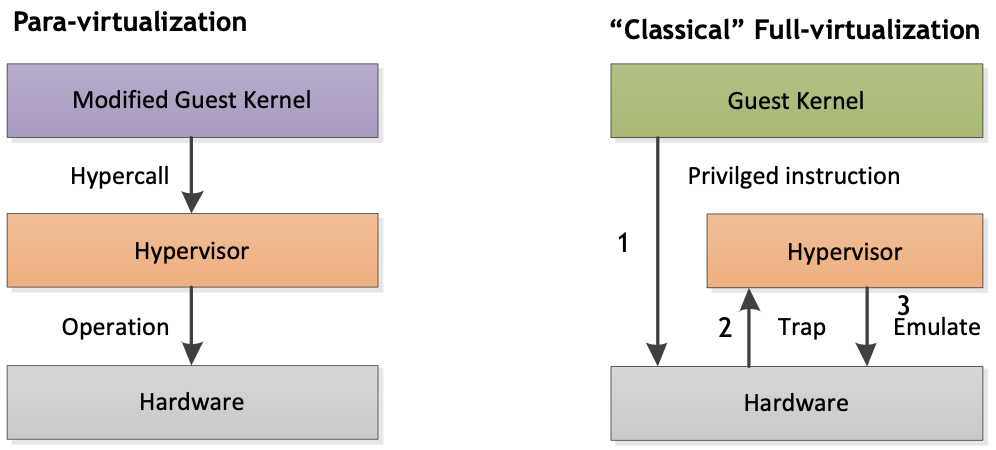
\includegraphics[width=0.3\textwidth]{img/img42.png}
    \caption{para vs full virtualization}
    \label{fig:para vs full}
    \end{center}
\end{figure}

\subsection{Containers}
\begin{defn}
    Containers are pre-configured packages, with everything you need to execute the code (code, libraries, variables and configurations) in the target machine.
\end{defn}
The main advantage of containers is that their behavior is predictable, repeatable and immutable:\\
when I create a "master" container and duplicate it on another server, I know exactly how it will be executed.There are no unexpected errors when moving it to a new machine or between environments.\\\\
Example: a container for a website,\\
• We are not required to export/import the development/test/production environments,\\
• We create a container that contains the site and bring it to the destination environment\\\\
\subsubsection{Containers and Virtual Machine}
VM provides hardware virtualization, while containers provide virtualization at the operating system level.\\
The \underline{main difference} is that the containers share the host system kernel with other containers.
\begin{figure}[H]
    \begin{center}
    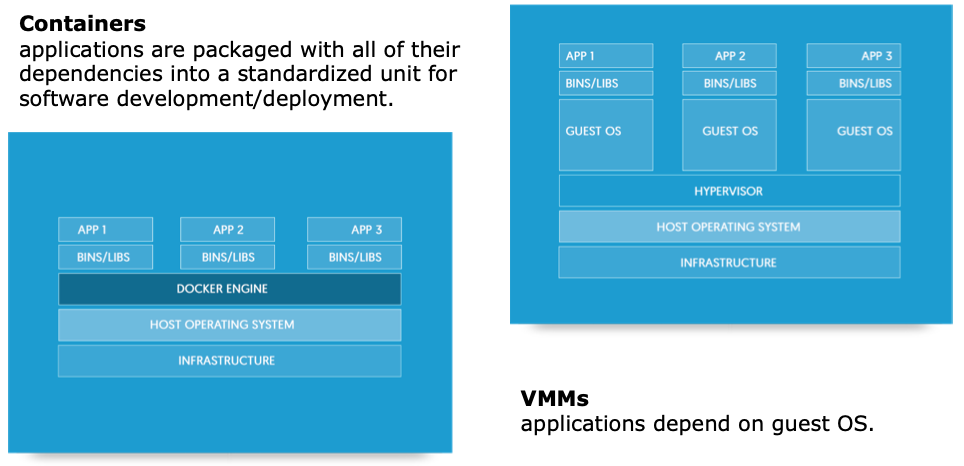
\includegraphics[width=0.5\textwidth]{img/img43.png}
    \caption{container vs VMMs}
    \label{fig:container vs VMMs}
    \end{center}
\end{figure}
\href{https://www.youtube.com/watch?v=cjXI-yxqGTI}{youtube video}
\subsubsection{Characteristics}
\begin{itemize}
    \item Flexible: even the most complex applications can be containerized;
    \item Light: the containers exploit and share the host kernel;
    \item Interchangeable: updates and updates can be distributed on the fly;
    \item Portable: you can create locally, deploy in the Cloud and run anywhere;
    \item Scalable: it is possible to automatically increase and distribute replicas of the container;
    \item Stackable: containers can be stacked vertically and on the fly.
\end{itemize}
Containers ease the deployment of applications and increase the scalability but they also impose a modular application development where the modules are independent and uncoupled.
\subsubsection{Usage}
\begin{itemize}
    \item Helping make your local development and build workflow faster, more efficient, and more lightweight.
    \item Running stand-alone services and applications consistently across multiple environments.
    \item Using Container to create isolated instances to run tests.
    \item Building and testing complex applications and architectures on a
    local host prior to deployment into a production environment.
    \item Building a multi-user Platform-as-a-Service (PAAS) infrastructure.
    \item Providing lightweight stand-alone sandbox environments for developing, testing, and teaching technologies, such as the Unix shell or a programming language.
    \item Software as a Service applications.
\end{itemize}

\newpage
\subsubsection{Software for “Containers”}
\begin{multicols}{2}
    \begin{figure}[H]
        \begin{center}
        
\includegraphics[width=0.4\textwidth]{img/img44.png}
        \caption{docker}
        \label{fig:docker}
        \end{center}
    \end{figure}
    \columnbreak
    \begin{itemize}
        \item Docker aims to create and distribute software inside containers.
        \item Open source platform of tools that helps to "build, ship and run
        any app, anywhere”
        \item Docker is based on a DockerFile (a textual file which contains all the commands that a user can call on the command line to assemble an image). DockerFiles define a compilation process which, if sent to the "Docker build" command, will produce an immutable docker image (a sort of snapshot of the application).
        \item It is possible to run the docker where the docker daemon is running: e.g., a laptop, a server, in the cloud or a Raspberry PI
        \item Regardless of where the image is running, the docker will behave in the same way.
        \item Docker Swarm is the container orchestration tool developed by Docker closely integrated within the Docker ecosystem
    \end{itemize}
\end{multicols}
\begin{multicols}{2}
    \begin{itemize}
        \item Kubernetes is a Google open source project
        \item Recommended for the management of medium and large clusters
        and complex applications;
        \item Extensive and customizable solution that allows you to coordinate large-scale node clusters in production more efficiently:\begin{itemize}
            \item Run containers on many heterogeneous machines;
            \item Increase or decrease the performance by proportionally
            modifying (adding or even removing) the containers
            \item Share the load between containers;
            \item Start new containers on different machines if a machine fails
        \end{itemize}
    \end{itemize}
    \columnbreak
    \begin{figure}[H]
        \begin{center}
        
\includegraphics[width=0.3\textwidth]{img/img45.png}
        \caption{kubernetes}
        \label{fig:kubernetes}
        \end{center}
    \end{figure}
\end{multicols}
\href{https://www.youtube.com/watch?v=2vMEQ5zs1ko}{youtube video}

\subsection{Theoretical Background: Popek and Goldberg}
Assumptions:
\begin{itemize}
    \item The hardware consists of a processor and a uniformly addressable memory (access time to a memory location is independent of which processor makes the request)
    \item The processor can operate in system mode (both system and user instructions) or user mode (only user instructions)
    \item A subset of the instruction set is available only in the system mode
    \item Memory addressing is done relative to the contents of a relocation register (i.e., a fixed value is added to a virtual address to arrive at a physical memory address).
    \item No I/O is considered (as I/O could be done in memory).
\end{itemize}The machine being virtualized is a 4-tuple:\\
{\bf S = $<$ E, M, P, R $>$}\begin{itemize}
    \item Executable Storage {\bf E} (conventional addressed memory of size q), i.e., the RAM
    \item Mode of Operation {\bf M}, i.e., User or System
    \item Program Counter {\bf P}
    \item Memory Relocation Bound Register {\bf R} is a pair (l, b)\begin{itemize}
        \item Physical location l of the virtual memory space
        \item Bound b, the size/extension of the virtual memory space
    \end{itemize}
\end{itemize}If the address a accessed by a program falls outside the bounds indicated by R, a {\sl memory trap} occurs.A context switch is performed:\begin{itemize}
    \item The current state of the machine is saved in location 0 (Current state is represented by values of (M,P,R))
    \item Copies the contents of location 0 of another process into M,P, and R. (Context switch)
\end{itemize}{\bf Instructions are then classified on the basis of their behavior as a function of the state S of the machine.}\\
\newline
Classifies the instructions of an ISA into 3 different (and possibly overlapping) groups based on their behavior:\begin{enumerate}
    \item {\bf Privileged} instructions: Those that trap if the processor is in user mode and do not trap if it is in system mode.\\E.g.:\begin{itemize}
        \item Load PSW (LPSW): load processor status word (PSW) if in system mode, from processor memory.\\
        Contains the P bit: specifies if the CPU is in user or system mode\\Critical for the control of the system!
        \item Set CPU timer (SPT): replaces the CPU interval timer if in system mode\\If executable in user mode, a user program could change the amount of time dedicated to it before swapping occour.
    \end{itemize}
To specify instructions that interact with hardware, two categories of special instructions are defined:
Could affect the correct functioning of the VMM because of their action. Divided into:
    \item {\bf Control sensitive }instructions: attempt to change the configuration of resources in the system.(e.g.: the physical memory assigned to a program)
    \item {\bf Behavior sensitive} instructions: those whose behavior or result depends on the configuration of resources (i.e.: the processor's mode affects the outcome)
\end{enumerate}
{\bf NOTE}: all of the guest OS software is hence forced to execute in user mode!
\subsubsection{Requirements}
System virtualization requires (requirements a VM must have to perform System-Level virtualization):\begin{itemize}
    \item Equivalence: A program running under the VMM should exhibit a behavior essentially identical to that demonstrated when running on an equivalent machine directly.
    \item Resource control: The VMM must be in complete control of the virtualized resources (guest cannot modify them).
    \item Efficiency: A statistically dominant fraction of machine instructions must be executed without VMM intervention.
\end{itemize}
{\bf Theorem}: for any conventional (third-generation) computer, a VMM may be constructed if the set of sensitive instructions for that computer is a subset of the set of privileged instructions (i.e., all the control/behavior instructions must be privileged)\\
\newline
To build a VMM it is sufficient that all instructions that could affect the correct functioning of the VMM (sensitive instructions) always trap and pass control to the VMM.\begin{itemize}
    \item Since the VM is in user mode, the execution of sensitive instructions will be trapped by the VMM
    \item \underline{This guarantees the resource control property.}
\end{itemize}
Non-privileged instructions must instead be executed natively (i.e.,
efficiently).\begin{itemize}
    \item \underline{This guarantees the efficiency property.}
\end{itemize}
Popek and Goldberg theorem provides the theoretical background for implementing a Virtual Machine Monitor using the trap-and-emulate virtualization.\\\\VMs always access the virtual resources using sensitive instructions.\\This allows to trap the guest system, call the VMM which in turn can emulate the resource.\begin{itemize}
    \item \underline{This ensures the equivalence property.}
\end{itemize}

\subsection{Implementing full virtualization}
\begin{multicols}{2}
    \begin{figure}[H]
        \begin{center}
        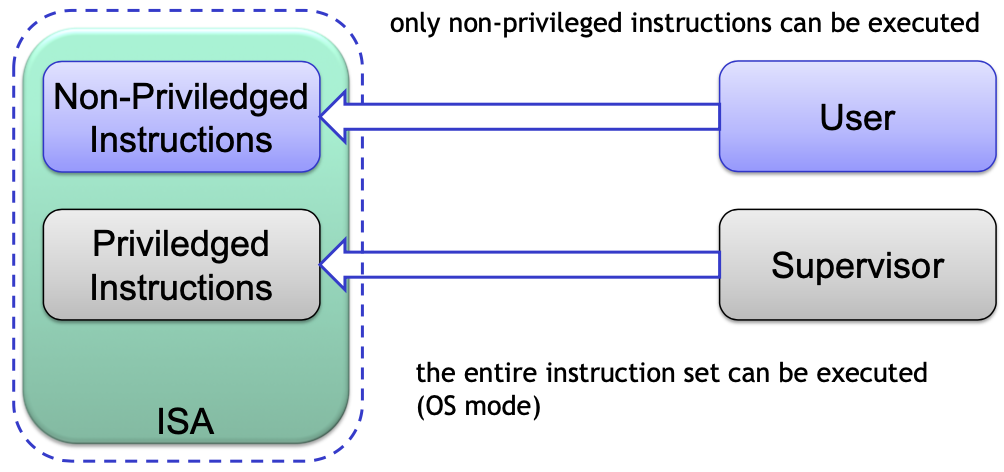
\includegraphics[width=0.3\textwidth]{img/img46.png}
        \caption{basic computer architecture}
        \label{fig:basic computer architecture}
        \end{center}
    \end{figure}
    \columnbreak
    The instruction set is divided into (at least) two categories: Non-Priviledged and Priviledged Instruuctions.\\\\A machine operates in two modes: User and Supervisor
\end{multicols}

\subsubsection{workflow}
\begin{multicols}{2}
    \begin{enumerate}
        \item The OS starts with the CPU in Supervisor mode.
        \item The OS using Supervisor privileged instructions defines the memory bounds where application will run.
        87
        \item The OS gives the control to the application, changing the CPU to User mode.
        \item The application runs normally using its non-privileged instructions.
        \item If the application tries to access memory outside the assigned bounds, the CPU traps them and return the control to the OS for stopping the application and prevent compromising the entire system.
    \end{enumerate}
    \columnbreak
    \begin{figure}[H]
        \begin{center}
        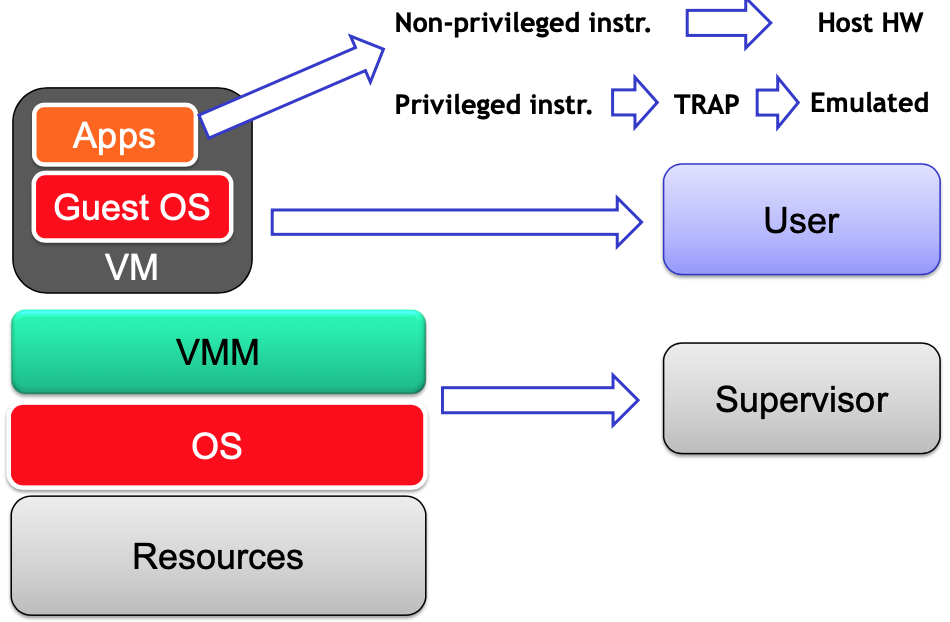
\includegraphics[width=0.4\textwidth]{img/img47.png}
        \caption{VM environments}
        \label{fig:VM environments}
        \end{center}
    \end{figure}
\end{multicols}
\newpage
\subsubsection{Hardware-Assisted}
Both AMD and Intel have modified their architectures to support virtualization Intel VT e AMD-V:\begin{multicols}{2}
    \begin{figure}[H]
        \begin{center}
        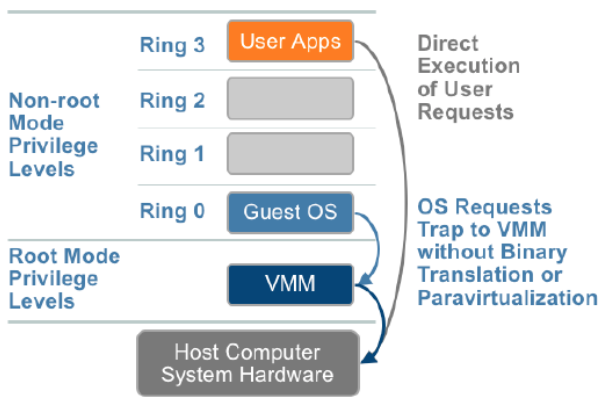
\includegraphics[width=0.35\textwidth]{img/img48.png}
        \caption{Hardware-Assisted}
        \label{fig:Hardware-Assisted}
        \end{center}
    \end{figure}\columnbreak
    \begin{itemize}
        \item a new high privilege ring for the VMM. (VMX root and VMX non-root)
        \item Hardware transitions from ring 0 to the VMM.
        \item Processor state is maintained
        for each guest OS (and the VMM) in separate
        address spaces
    \end{itemize}
\end{multicols}
\subsubsection{Root operation}
Two modes of operation for the processor:\begin{itemize}
    \item VMX root operation (VMM)\begin{itemize}
        \item Processor behaves as would have if no VT-x
        \item Can use a whole set of instructions called VMX
    \end{itemize}
    \item VMX non-root operation (VM)\begin{itemize}
        \item Processor limited: critical shared resources are kept under the control
        of a monitor running in VMX root operation.
        \item Limitation extended also to the ring 0!   
    \end{itemize}
\end{itemize}
Both support privilege levels 0-3.\\
Guest software can run in the rings in which it was originally intended to be run: guest OS believes it is running at level 0
\subsubsection{Transitions}
\begin{figure}[H]
    \begin{center}
    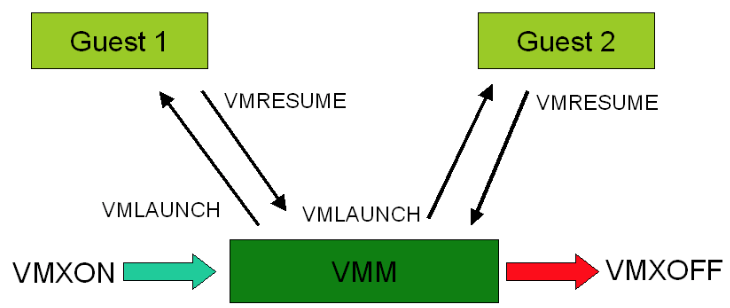
\includegraphics[width=0.4\textwidth]{img/img49.png}
    \caption{Transitions}
    \label{fig:Transitions}
    \end{center}
\end{figure}
VMXON instructions transfer control to VM: state restore from VMCB\\
Exits occur based on the content of the VMCB\begin{itemize}
    \item State saved to VMCB
    \item Exit codes stored in VMCB to simplify VMM\\
    (E.g., exit due to I/O provide the port number\\
    E.g., exit due to page fault provide faulting address and access mode)
\end{itemize}
\newpage
%------------------------------------------------------------------------%

\section{Cloud Computing}
\subsection{Migration from Physical to Virtual}
\subsection*{Without virtualization:}\begin{itemize}
    \item Software strongly linked/related with hardware: move/change an application not a easy task
    \item To isolate failure/crash the classical model is:\begin{itemize}
        \item 1 server
        \item 1 operative system (OS)
        \item 1 application, with a resulting low CPU utilization (10-15\%)
    \end{itemize} • 
    \item Low flexibility
\end{itemize}
\subsection*{With Virtualization:}
\begin{itemize}
    \item Hw-independence: software/hardware no longer strongly related
    \item High fexibility thanks to pre-built VMs
    \item OS and applications can be handled as a «single entity»
\end{itemize}
{\bf Consolidation Management}: migration from physical to virtual machines, servers are connected one another so it is possible to:\begin{itemize}
    \item move Virtual Machines, without interrupting the applications running inside ({\bf scalability})
    \item automatically balances the Workloads according to set limits and guarantees ({\bf automatic scalability})
    \item Servers and Applications are protected against component and system failure ({\bf high availability})
\end{itemize}
\subsection*{Advantages of consolidations}
\begin{itemize}
    \item Different OS can run on the same hardware
    \item Higher hardware utilization\begin{itemize}
        \item Less hardware is needed (Acquiring costs, Management costs(human resources, power, cooling))
        \item Green IT-oriented
    \end{itemize} 
    \item Continue to use legacy software (e.g., software for WIN on Linux machines thanks to VMs)
    \item Application independent from the hardware
\end{itemize}

\subsection{Cloud Computing}
\begin{defn}
    Cloud computing is a model for enabling\begin{itemize}
        \item convenient
        \item on-demand
    \end{itemize}network access to a shared pool of configurable computing
    resources, like for example: Networks, Servers, Storage, Applications and Services\\
    that can be rapidly provisioned and released with minimal management effort or service provider interaction.
\end{defn}
\begin{figure}[H]
    \begin{center}
    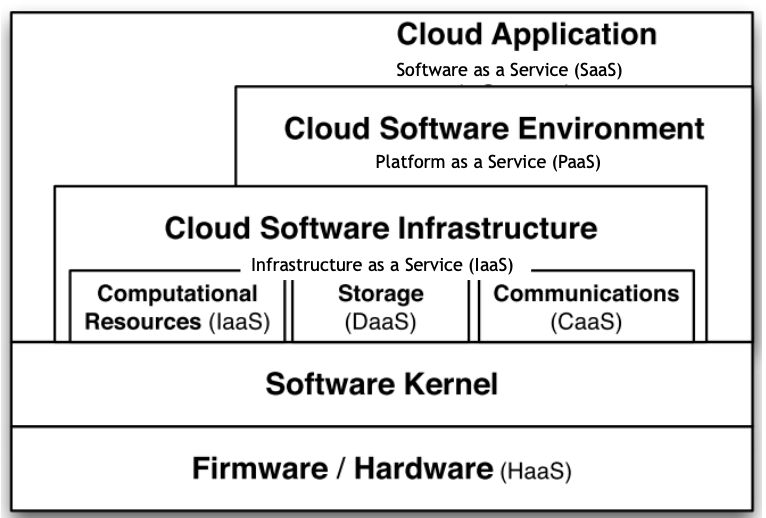
\includegraphics[width=0.5\textwidth]{img/img50.png}
    \caption{Cloud computing}
    \label{fig:Cloud computing}
    \end{center}
\end{figure}

\subsubsection{Cloud Application Layer}
{\bf SaaS} (Software as a Service)\\
Users access the services provided by this layer through web-portals,
and are sometimes required to pay fees to use them.\\
Cloud applications can be developed on the cloud software environments or infrastructure components.\\\\
Example: GMail, Google Docs and related apps (online office), SalesForce.com (CRMaaS)

\subsubsection{Cloud Software Environment Layer}
{\bf PaaS} (Platform as a Service)\\
Users are application developers.\\
Providers supply developers with a programming-language-level environment with well-defined a API\begin{itemize}
    \item Facilitate interaction between environment and apps  \item Accelerate the deployment
    \item Support scalability
\end{itemize}
Examples in Deep Learning: Amazon SageMaker, Microsoft Azure Machine Learning, Google AI: TensorFlow
\subsubsection{Cloud Software Infrastructure Layer}
Provides resources to the higher-level layers (i.e., Software and Software Environment)
Note that Cloud Apps and Cloud SW might bypass Cloud SW Infrastructure: However, this would reduce\begin{itemize}
    \item Simplicity
    \item Development efforts
\end{itemize} 
\subsubsection*{Computational Resources}
{\bf IaaS} (Infrastructure or Integration as a Service)
\begin{multicols}{2}
    {\bf VM's benefits}\begin{itemize}
        \item Flexibility
        \item Super-user (root) access to VM for fine granularity settings and customization of installed sw
    \end{itemize}
    \columnbreak
    {\bf VM's issues}\begin{itemize}
        \item Performance interference
        \item Inability to provide strong guarantees about SLAs
    \end{itemize}
\end{multicols}
Examples:\begin{itemize}
    \item Commercial solutions\begin{itemize}
        \item Amazon Elastic Cloud (EC2): Full virtualization + Based on Xen 
        \item Windows Azure. (Not just windows-based: it allows also to start VMs for other OSs.)  
        \item Google Compute Engine. (Same infrastructure as Google.)
        \item Rackspace Open Cloud.
        \item IBM SmartCloud Enterprise.
        \item HP Enterprise Converged Infrastructure.
    \end{itemize}
    \item Open-source projects\begin{itemize}
        \item Eucalyptus Systems  \item Apache CloudStack 
        \item Open Stack: The project aims to deliver solutions for all types of clouds (private or public) by being simple to implement, massively scalable, and feature rich.
    \end{itemize}
\end{itemize}

\subsubsection*{Storage}
{\bf DaaS} (Data as a Service)\\
Allows users to store their data at remote disks and access data anytime from any place.\\
Facilitates cloud applications to scale beyond their limited servers requirements:\begin{itemize}
    \item High dependability: availability, reliability, performance (scalability)
    \item Replication
    \item Data consistency
\end{itemize}
Examples: DropBox, iCloud, GoogleDrive.\\CEPH is an open source solution.

\subsubsection*{Communications}
{\bf CaaS} (Communication as a Service)\\Communications becomes a vital component in guaranteeing QoS.\\\\CaaS is part of a larger category of services known as software as a service (SaaS), in which vendors offer software products and services over the Internet.\\The core concept of CaaS is that accessing these services over the internet is extremely convenient.\\\\Types of CaaS include Voice over Internet Protocol (VoIP) or internet telephone solutions, and video conferencing services.

\subsection{Types of Clouds}
\begin{figure}[H]
    \begin{center}
    \includegraphics[width=0.5\textwidth]{img/img51.png}
    \caption{Cloud types}
    \label{fig:Cloud types}
    \end{center}
\end{figure}
\subsubsection{Public}
Large scale infrastructure available on a rental basis\begin{itemize}
    \item Operating System virtualization (e.g. Xen) provides CPU isolation
    \item “Roll-your-own” network provisioning provides network isolation
    \item Locally specific storage abstractions
\end{itemize}
Fully customer self-service\begin{itemize}
    \item Service Level Agreements (SLAs) are advertized
    \item Requests are accepted and resources granted via web services
    \item Customers access resources remotely via the Internet
\end{itemize}
Accountability is e-commerce based\begin{itemize}
    \item Web-based transaction
    \item “Pay-as-you-go” and flat-rate subscription  
    \item Customer service, refunds, etc.
\end{itemize}

\subsubsection{Private}
Internally managed data centers\\
The organization sets up a virtualization environment on its own servers: in its data center or in the data center of a managed service provider\\Key benefits:\begin{itemize}
    \item you have total control over every aspect of the infrastructure
    \item you gain advantages of virtualization
\end{itemize}
Issue: It lacks the freedom from\begin{itemize}
    \item capital investment
    \item Flexibility (“almost infinite” grow of cloud computing)
\end{itemize}Useful for companies that have significant existing IT investments

\subsubsection{Community}
A single cloud managed by several federated organizations.\\Combining together several organizations allows economy of scale.\\Resources can be shared and used by one organization, while the others are not using them.\\\\Technically similar to private cloud: they share the same software and the same issues but a more complex accounting system is however required.\\Hosted locally or externally:\begin{itemize}
    \item Typically community clouds shares infrastructures of the participants.
    \item However they can be hosted by a separate specific organization, or only by a small subset of the partners.
\end{itemize}

\subsubsection{Hybrid}
Hybrid clouds are the combination of any of the previous types: usually are companies that holds their private cloud, but that they can be subject to unpredictable peaks of load. In this case, the company rents resources from other types of cloud.\\Common interfaces\begin{itemize}
    \item To simplify the deployment process, the way in which VMs are started, terminated, address is given and storage is accessed, must be as similar as possible.
    \item Many standards are being developed in this directions, but none is globally accepted yet.
    \item Currently, the Amazon EC2 model is the one with more compliant infrastructures.
\end{itemize}

\begin{multicols}{2}
    \subsection{Advantages of Cloud Computing}
Cloud computing has many positive aspects:\begin{itemize}
    \item Lower IT costs
    \item Improved performance
    \item Instant software updates
    \item “Unlimited” storage capacity
    \item Increased data reliability
    \item Universal document access
    \item Device Independence
\end{itemize}
\columnbreak
\subsection{Disdvantages of Cloud Computing}
However, it can also have some disadvantages:\begin{itemize}
    \item Requires a constant Internet connection
    \item Does not work well with low-speed connections
    \item Features might be limited
    \item Can be slow
    \item Stored data might not be secure
    \item Stored data can be lost
\end{itemize}
\end{multicols}


\subsection{Fog/Edge Computing}
\begin{multicols}{2}
    It stays in the middle between the objects and the cloud: the computation is split. The fog pre-processes the data and, if it is able, it takes a decision, otherwise it sends them to the cloud to exploit its major computation power.
    \columnbreak
    \begin{figure}[H]
        \begin{center}
        \includegraphics[width=0.4\textwidth]{img/img52.png}
        \caption{Fog and Edge Computing}
        \label{fig:Fog/Edge Comp}
        \end{center}
    \end{figure}
\end{multicols}

\newpage
%------------------------------------------------------------------------%
\section{Machine Learning as a service}
\begin{multicols}{2}
    \begin{figure}[H]
        \begin{center}
        \includegraphics[width=0.4\textwidth]{img/img53.png}
        \caption{IT perspective for AI}
        \label{fig:IT perspective for AI}
        \end{center}
    \end{figure}
    \columnbreak
    \begin{figure}[H]
        \begin{center}
        \includegraphics[width=0.3\textwidth]{img/img54.png}
        \caption{IT architecture for ML/DL}
        \label{fig:IT architecture for ML/DL}
        \end{center}
    \end{figure}
\end{multicols}

\begin{multicols}{2}
    \subsection{Computing Cluster}
    \begin{itemize}
        \item Servers (parallelelization and scalability are key to find the best model as well as HW accelerators):\\
        • General Purpose CPU\\
        • GPU (TPU)
        \item Storage (multiple storage systems including
        distributed/parallel file systems):\\
        • DirectAttachedStorage\\
        • NAS\\
        • SAN\\
        \item Network (applications are generally non-iterative):\\ • Ethernet
    \end{itemize}
    \subsection{Virtual Machine Manager}\begin{itemize}
        \item Virtualization is carried out through hypervisor (virtual machines) or containers
        \item Resources are increased by adding more virtual machines (provided that hardware resources are available)
        \item User can design personalized software environments and scale instances to the needs
    \end{itemize}Some examples: VMware, Xen, KVM, HyperX, Kubernetes
    \columnbreak
    \subsection{Computing Framework}
    Computing Frameworks are composed by several modules:\begin{itemize}
        \item Cluster Manager
        \item Data Storage
        \item Data processing engine
        \item Graph computation
        \item Programming Languages (Java, Python, Scala, R)
    \end{itemize}
    An application (e.g., a big-data application) operating in a cluster is distributed among different computing (virtual) machines.\\
    Examples:\begin{itemize}
        \item Computing Framework: Hadoop, Spark, Flink
        \item Scheduling: Apache Mesos, Hadoop YARN
        \item Storage: HDFS, Hbase, Amazon S3, Cassandra, Mongo DB, Spark SQL
        \item Data Processing Engine: Spark, Map-Reduce
    \end{itemize}
    \subsection{Machine/Deep Learning Framework}
    \begin{itemize}
        \item \underline{Machine learning frameworks} cover a variety of learning methods for classification, regression, clustering, anomaly detection, and data preparation, and it may or may not include neural network methods.
        \item \underline{Deep learning frameworks} cover a variety of neural network topologies with many hidden layers.
    \end{itemize}
    \begin{figure}[H]
        \begin{center}
        \includegraphics[width=0.3\textwidth]{img/img55.png}
        \caption{ML/DL frameworks}
        \label{fig:ML/DL frameworks}
        \end{center}
    \end{figure}
\end{multicols}

Cloud comuputing simplifies the access to ML capabilities for\begin{itemize}
    \item designing a solution (without requiring a deep knowledge of ML)
    \item setting up a project (managing demand increases and IT solution)
\end{itemize}
To support ML in the Cloud companies as Amazon, Microsoft and Google provide\begin{figure}[H]
    \begin{center}
    \includegraphics[width=0.5\textwidth]{img/img56.png}
    \end{center}
\end{figure}
\begin{multicols}{3}
    \begin{figure}[H]
        \begin{center}
        \includegraphics[width=0.3\textwidth]{img/img57.png}
        \caption{ML Infrastructure as a Service}
        \end{center}
    \end{figure}
    \columnbreak
    \begin{figure}[H]
        \begin{center}
        \includegraphics[width=0.3\textwidth]{img/img58.png}
        \caption{ML Platform as a Service}
        \end{center}
    \end{figure}
    \columnbreak
    \begin{figure}[H]
        \begin{center}
        \includegraphics[width=0.3\textwidth]{img/img59.png}
        \caption{ML software as a Service}
        \end{center}
    \end{figure}
\end{multicols}

\begin{multicols}{2}
    \subsection*{Pros}
    Cloud computing simplifies the access to ML/DL capabilities for\begin{itemize}
        \item designing a
        solution (without requiring a deep knowledge of ML/DL)
        \item setting up a project (managing
        demand increases and IT solution)
    \end{itemize}
    \columnbreak
    \subsection*{Cons}
    \begin{itemize}
        \item Internet connection
        \item High Power
        Consumption
        \item Privacy and Security
        \item Latency in making
        decision
    \end{itemize}
\end{multicols}
Machine and Deep Learning plaforms for IoT and Edge\begin{itemize}
    \item Increase autonomy
    \item Reduce decision-making latency 
    \item Reduce transmission bandwidth 
    \item Increase energy-efficiency
    \item Security and Privacy
\end{itemize}
\begin{multicols}{2}
    \begin{figure}[H]
        \begin{center}
        \includegraphics[width=0.4\textwidth]{img/img60.png}
        \end{center}
    \end{figure}
    \columnbreak
    \begin{figure}[H]
        \begin{center}
        \includegraphics[width=0.4\textwidth]{img/img61.png}
        \end{center}
    \end{figure}
\end{multicols}
\newpage

%------------------------------------------------------------------------%
\section{RAID}
\subsection*{Redundant Arrays of Independent (Inexpensive) Disks}
\underline{Disk Arrays}: proposed in the 1980’s [PATTERSON].\\
Need to increase the {\bf performance}, the {\bf size} and the {\bf reliability} of storage systems.\\\\
Several {\sl independent} disks that are considered as a single, large,high-performance logical disk (In contrast with the JBOD (Just a Bunch of Disks) method where each disk is a separate device with a different mount point)\\
The data are {\sl striped} across several disks accessed in parallel:\begin{itemize}
    \item high data transfer rate: large data accesses (heavy I/O op.)
    \item high I/O rate: small but frequent data accesses (light I/O op.)
    \item load balancing across the disks
\end{itemize}
Two orthogonal techniques:\begin{enumerate}
    \item {\bf data striping}: to improve performance
    \item {\bf redundancy}: to improve reliability
\end{enumerate}

\subsection{Data striping}
\begin{defn}
    {\bf Striping}: data are written sequentially (a vector, a file, a table, ...) in units (stripe unit: bit, byte, blocks) on multiple disks according to a cyclic algorithm ({\sl round robin})
\end{defn}
\begin{defn}
    {\bf stripe unit}: dimension of the unit of data that are written on a single disk
\end{defn}
\begin{defn}
    {\bf stripe width}: number of disks considered by the striping algorithm
\end{defn}\begin{enumerate}
    \item multipleindependentI/Orequestswillbeexecutedin parallel by several disks decreasing the queue length (and time) of the disks
    \item single multiple-block I/O requests will be executed by multiple disks in parallel increasing of the transfer rate of a single request
\end{enumerate}

\subsection{Redundancy}
The main {\bf motivation} for the introduction of redundancy: the more physical disks in the array, the larger the size and performance gains; but... the larger the probability of failure of a disk!\\\\The probability of a failure (assuming independent failures) in an array of 100 disks is 100 higher the probability of a failure of a single disk\\(if a disk has an Mean Time To Failure (MTTF) of 200,000 hours (~23 years) an array of 100 disks will show a MTTF of 2000 hours (~ 3 months))
\begin{defn}
    {\bf Redundancy}: error correcting codes (stored on disks different from the ones with the data) are computed to tolerate loss due to disk failures
\end{defn}Since write operations must update also the redundant information,their performance is worse than the one of the traditional writes.
\subsection{Disks}
Hard drives are great devices: relatively fast, persistent storage. But them have also limitations:\begin{itemize}
    \item How to cope with disk failure? Mechanical parts may break over time and sectors may become silently corrupted
    \item Capacity is limited: managing files across multiple physical devices is cumbersome (can we make 10x 1 TB drives look like a 10 TB drive?)
\end{itemize}
\begin{defn}
    {\bf RAID}: use multiple disks to create the illusion of a large, faster, more reliable disk
\end{defn}
\subsection{Externally}
It looks like a single disk:
\begin{itemize}
    \item RAID is transparent
    \item Data blocks are read/written as usual
    \item No need for software to explicitly manage multiple disks or perform error checking/recovery
\end{itemize}
\subsection{Internally}
It is a complex computer system:
\begin{itemize}
    \item Disks managed by a dedicated CPU + software 
    \item RAM and non-volatile memory
    \item Many different configuration options ( RAID levels )
\end{itemize}
\subsection{Levels}
\begin{itemize}
    \item RAID 0 striping only
    \item RAID 1 mirroring only\\ RAID 0+1 (nested levels)\\ RAID 1+0 (nested levels)
    \item {\color{lightgray}RAID 2 bit interleaving (not used)}
    \item {\color{lightgray}RAID 3 byte interleaving - redundancy (parity disk)}
    \item RAID 4 block interleaving - redundancy (parity disk)
    \item RAID 5 block interleaving - redundancy (parity block distributed)
    \item RAID 6 greater redundancy (2 failed disks are tolerated)
\end{itemize}

\subsubsection{Level 0}
\subsubsection*{Striping, no redundancy}
\begin{multicols}{2}
    Data are written on a single logical disk and splitted in several blocks distributed across the disks according to a striping algorithm.\\\\Used where {\bf performance} and {\bf capacity} (rather than {\sl reliability}) are the primary concerns, minimum two drivers required.\\\\
\underline{lowest cost} because it does not employ redundacy (no error correcting codes are computed and stored)\\
\underline{best write performance} it does not need to update redundant data and it is parallelized\\
single disk failure will result in \underline{data loss}\columnbreak
\begin{figure}[H]
    \begin{center}
    \includegraphics[width=0.5\textwidth]{img/img62.png}
    \caption{RAID level 0}
    \end{center}
\end{figure}
\end{multicols}
\subsubsection*{Striping}
Key idea: present an array of disks as a single large disk.\\
Maximize parallelism by striping data cross all N disks.\begin{figure}[H]
    \begin{center}
    \includegraphics[width=0.5\textwidth]{img/img63.png}
    \end{center}
\end{figure}
\subsubsection*{Addressing Blocks}
How do you access specific data blocks?\\
{\bf Disk} = logical block number \% number of disks\\
{\bf Offset} = logical block number / number of disks\\
Example: read block 11\begin{itemize}
    \item 11\%4=Disk3
    \item 11 / 4 = Physical Block 2 (starting from 0)
\end{itemize}
\subsubsection*{Chunk Sizing}
\begin{figure}[H]
    \begin{center}
    \includegraphics[width=0.4\textwidth]{img/img64.png}
    \end{center}
\end{figure}

\subsubsection*{Performance}
As usual, we focus on sequential and random workloads
\begin{figure}[H]
    \begin{center}
    \includegraphics[width=0.4\textwidth]{img/img65.png}
    \end{center}
\end{figure}
\begin{itemize}
    \item Assume disks in the array have sequential transfer rate S.\\Single large transfer:\begin{itemize}
        \item 10 MB transfer
        \item S = transfer size / time to access
        \item 10MB/(7ms+3ms+10MB/50MB/s)=47.62MB/s
    \end{itemize}
    \item Assume disks in the array have random transfer rate R.\\Set of small files:\begin{itemize}
        \item 10 KB transfer
        \item R = transfer size / time to access
        \item 10KB/(7ms+3ms+10KB/50MB/s)=0.98MB/s
    \end{itemize}
\end{itemize}
{\bf Capacity}: N\\  All space on all drives can be filled with data\\\\
{\bf Reliability}: O\\  If any drive fails, data is permanently lost\\  MTTDL = MTTF\\\\
{\bf Sequential read and write}: N*S\\  Full parallelization across drives\\\\
{\bf Random read and write}: N*R\\ Full parallelization across all drives

\subsubsection{Level 1}
\begin{multicols}{2}
    \subsubsection*{Mirroring}
    Whenever data is written to a disk it is also duplicated (mirrored) to a second disk (there are always {\bf two copies} of the data), minimum 2 disk drives.\\\\
    \underline{high reliability}:when a disk fails the second copy is used\\
    \underline{read of a data}: it can be retrieved from the disk with the shorter queueing, seek, and latency delays\\
    \underline{fast writes} (no error correcting code should be computed)but still slower than standard disks (due to duplication)\\
    \underline{high costs} 50 \% of the capacity isused
    \columnbreak
    \begin{figure}[H]
        \begin{center}
        \includegraphics[width=0.3\textwidth]{img/img66.png}
        \caption{RAID Level 1}
        \end{center}
    \end{figure}
\end{multicols}
\subsubsection*{Mirroring}
\begin{multicols}{2}
    In principle, a RAID 1 can mirror the content over more than one disk.\begin{itemize}
        \item This give resiliency to errors even if more than one disk breaks
        \item It allows with a voting mechanism to identify errors not reported by the disk controller.
    \end{itemize}
    In practice this is never used, because the overhead and costs are too high.\\RAID 0 offers high performance, but zero error recovery. Key idea: make two {\bf copies} of all data.
    \columnbreak
    \begin{figure}[H]
        \begin{center}
        \includegraphics[width=0.33\textwidth]{img/img67.png}
        \end{center}
    \end{figure}
\end{multicols}However if several disks are available (always in an {\sl even} number), disks could be coupled.\\{\sl The total capacity is halved}.\\Each disk has a mirror; How to organize this? RAID levels can be combined: Raid0+1   Raid1+0
\newpage
\begin{multicols}{2}
    \begin{figure}[H]
        \begin{center}
        \includegraphics[width=0.4\textwidth]{img/img68.png}
        \end{center}
    \end{figure}
    \columnbreak
    RAID levels can be {\bf combined}\\RAID x + y (or xy):\begin{itemize}
        \item {\sl n x m} disks in total
        \item Consider \underline{m groups} of \underline{n disks}
        \item Apply RAID x to each group of n disks
        \item Apply RAID y considering the m groups as single disks
    \end{itemize}
\end{multicols}
\begin{multicols}{2}
    \subsubsection{Level 0 + 1}
    \begin{figure}[H]
        \begin{center}
        \includegraphics[width=0.5\textwidth]{img/img69.png}
        \end{center}
    \end{figure}
    \columnbreak
    \subsubsection{Level 1 + 0}
    \begin{figure}[H]
        \begin{center}
        \includegraphics[width=0.5\textwidth]{img/img70.png}
        \end{center}
    \end{figure}
\end{multicols}
\begin{multicols}{2}
    \begin{figure}[H]
        \begin{center}
        \includegraphics[width=0.3\textwidth]{img/img71.png}
        \caption{0+1 and 1+0 organizations}
        \end{center}
    \end{figure}\columnbreak
    The blocks are the same but are allocated in a different order\\{\bf Performance} on both RAID 10 and RAID 01 are the same.\\The {\bf storage capacity} of RAID 10 and RAID 01 is the same.\\The main difference is the {\bf fault tolerance} level: for RAID 0+1 is less, for RAID 1+0 is larger.
\end{multicols}
{\bf Capacity}: N / 2\\  Two copies of all data, thus half capacity\\\\
{\bf Reliability}: 1 drive can fail, sometime more\\  If you are lucky, N / 2 drives can fail without data loss\\\\
{\bf Sequential write}: (N/2)*S\\  Two copies of all data, thus half throughput\\\\
{\bf Sequential read}: (N/2)*S\\ Half of the read blocks are wasted, thus halving throughput\\\\
{\bf Random read}: N*R\\  Best case scenario for RAID 1\\ Reads can parallelize across all disks
\\\\
{\bf Random write}: (N/2)*R\\ Two copies of all data, thus half throughput\\\\
\subsubsection*{The Consistent Update Problem}Mirrored writes should be atomic (All copies are written, or none are written); However, this is difficult to guarantee (Example: power failure)\\
Many RAID controllers include a
{\bf write-ahead log}\begin{itemize}
    \item Battery backed, non-volatile storage of pending writes
    \item A recovery procedure ensures to recover the out-of-sync mirrored copies
\end{itemize}
\subsubsection*{Decreasing the Cost of Reliability}RAID 1 offers highly reliable data storage but, it uses N / 2 of the array capacity; \\We can achieve the same level of reliability without wasting so much capacity: use information coding techniques to build light-weight error recovery mechanisms!

\subsubsection{Level 4}
\subsubsection*{Party Drive}
\begin{figure}[H]
    \begin{center}
    \includegraphics[width=0.5\textwidth]{img/img72.png}
    \caption{RAID level4}
    \end{center}
\end{figure}
\subsubsection*{Write}
\begin{enumerate}
    \item Additive parity
    \begin{figure}[H]
        \begin{center}
        \includegraphics[width=0.35\textwidth]{img/img73.png}
        \end{center}
    \end{figure}
    \item Subtractive parity
    \begin{figure}[H]
        \begin{center}
        \includegraphics[width=0.35\textwidth]{img/img74.png}
        \end{center}
    \end{figure}
\end{enumerate}
\subsubsection*{Read}
\begin{multicols}{2}
Reads (Serial or Random) are not a problem in RAID4\\ Parallelization across all non-parity blocks in the stripe
\columnbreak
\begin{figure}[H]
    \begin{center}
    \includegraphics[width=0.4\textwidth]{img/img75.png}
    \end{center}
\end{figure}
\end{multicols}\
\begin{multicols}{2}
    \subsubsection*{Serial Writes}
    RAID 4 has the same Read and Write write performance.\\Parallelization across all non-parity blocks in the stripe.\begin{figure}[H]
        \begin{center}
        \includegraphics[width=0.4\textwidth]{img/img76.png}
        \end{center}
    \end{figure}
    \columnbreak
    \subsubsection*{Random Writes}
    \begin{enumerate}
        \item Read the target block and the parity block
        \item Use subtraction to calculate the new parity block
        \item Write the target block and the parity block
    \end{enumerate}
    RAID 4 has terrible write performance: Bottlenecked by the parity drive
    \begin{figure}[H]
        \begin{center}
        \includegraphics[width=0.4\textwidth]{img/img77.png}
        \end{center}
    \end{figure}
\end{multicols}
{\bf Capacity}: N - 1\\  Space on the parity drive is lost\\\\
{\bf Reliability}: 1 drive can fail\\  Massive performance degradation during partial outage\\\\
{\bf Sequential read and write}: (N-1)*S\\  Parallelization across all non-parity blocks in the stripe\\\\
{\bf Random read}: (N-1)*R\\  Reads parallelize over all but the parity drive\\\\
{\bf Random write}: R/2\\  Writes serialize due to the parity drive
\\ Each write requires 1 read and 1 write of the parity drive, thus R / 2\\\\

\subsubsection{Level 5}
\subsubsection*{Rotating Party}
\begin{figure}[H]
    \begin{center}
    \includegraphics[width=0.5\textwidth]{img/img78.png}
    \caption{RAID level4}
    \end{center}
\end{figure}
\subsubsection*{Random Writes}
\begin{enumerate}
    \item Read the target block and the parity block
    \item Use subtraction to calculate the new parity block
    \item Write the target block and the parity block
\end{enumerate}
Thus, 4 total operations (2 reads, 2 writes); Distributed across all drives
\begin{figure}[H]
    \begin{center}
    \includegraphics[width=0.4\textwidth]{img/img79.png}
    \end{center}
\end{figure}{\bf Capacity}: N - 1 [same as RAID4]\\\\
{\bf Reliability}: 1 drive can fail [same as RAID4]\\  Massive performance degradation during partial outage\\\\
{\bf Sequential read and write}: (N-1)*S [same as RAID4]\\  Parallelization across all non-parity blocks in the stripe\\\\
{\bf Random read}: N*R [vs (N-1)*R]\\  Reads parallelize over all drives\\\\
{\bf Random write}: N/4 [vs R/2]\\  Writes parallelize over all drives\\ Each write requires 2 reads and 2 write, hence N / 4\\\\
{\bf N} = number of drives\\
{\bf R} = random access speed\\
{\bf S} = sequential access speed\\
{\bf D} = latency to access a single disk
\begin{figure}[H]
    \begin{center}
    \includegraphics[width=0.3\textwidth]{img/img80.png}
    \caption{Comparison of levels}
    \end{center}
\end{figure}

\subsubsection{Level 6}
More fault tolerance with respect RAID5.\\
2 concurrent failures are tolerated.\\
Uses Solomon-Reeds codes with two redundancy schemes : (P+Q) distributed and independent.\\
N + 2 disks required.\\
High overhead for writes (computation of parities): each write require 6 disk accesses due to the need to update both the P and Q parity blocks (slow writes).\\
Minimum set of 4 data disks
\begin{figure}[H]
    \begin{center}
    \includegraphics[width=0.4\textwidth]{img/img81.png}
    \end{center}
\end{figure}

\subsubsection{Level comparison}
Best performance and most capacity? -$>$ RAID 0\\
Greatest error recovery? -$>$ RAID 1 (1+0 or 0+1) or RAID 6\\
Balance between space, performance, and recoverability? -$>$ RAID 5\begin{figure}[H]
    \begin{center}
    \includegraphics[width=0.5\textwidth]{img/img82.png}
    \end{center}
\end{figure}

\subsection{Other Considerations}
\subsubsection{Many RAID systems include a hot spare}\begin{itemize}
    \item An idle, unused disk installed in the system
    \item If a drive fails, the array is immediately rebuilt using the hot spare
\end{itemize}
\subsubsection{RAID can be implemented in hardware or software}\begin{itemize}
    \item Hardware is faster and more reliable...
    \item But, migrating a hardware RAID array to a different hardware controller almost never works
    \item Software arrays are simpler to migrate and cheaper, but have worse performance and weaker reliability (Due to the consistent update problem)
\end{itemize}


%------------------------------------------------------------------------%

\end{document}
